\documentclass[a4paper, 11pt, onecolumn, oneside]{report}

\setcounter{tocdepth}{3} % Para aparecer no índice subsubsections
\setcounter{secnumdepth}{3} % Para subsubsections serem numeradas

%%%%% Funcionalidades %%%%%
\usepackage[T1]{fontenc} % Fontes T1
\usepackage[utf8]{inputenc} % Input UTF8
\usepackage[backend=biber, style=ieee]{biblatex} % para usar bibliografia
\usepackage{csquotes}
\usepackage[portuguese]{babel} %Usar língua portuguesa
\usepackage{blindtext} % Gerar texto automaticamente
\usepackage[printonlyused]{acronym}
\usepackage{hyperref} % para autoref
\usepackage{wrapfig} % Imagens junto do texto
\usepackage{graphicx}
\usepackage{indentfirst}
\usepackage{float}
\usepackage{geometry}
\usepackage{titlesec} % Package to customize section titles

\newcommand{\coo}{\ensuremath{\mathrm{CO_2}}}

\setlength{\fboxsep}{0pt}  % Remove o espaço entre a imagem e a borda
\setlength{\fboxrule}{1pt}  % Define a espessura da borda

\bibliography{bibliografia}
\graphicspath{{images/}} % Diretório com as Imagens

% Customize chapter format to prevent new page
\titleformat{\chapter}[block]{\normalfont\huge\bfseries}{\thechapter}{1em}{}
\titlespacing*{\chapter}{0pt}{0pt}{20pt}

%%%%%%%%%%%%%%%%%%%%%%%%%%%%%%%%%%%%%%%%%%%%%%%%%%%%%%%%
\begin{document}
%%
% Definições
%
\def\titulo{Ações Climáticas}
\def\data{DATA}
\def\autores{Martim Gomes, Tiago Fernandes, Tiago Mendes, Tiago Vieira}
\def\autorescontactos{\textbf{Email Contacto: }tiagoafernandes@ua.pt}
\def\departamento{119488, 120271, 119378, 119655 - Dpt. de Eletrónica, Telecomunicações e Informática}
\def\empresa{Universidade de Aveiro}
\def\logotipo{ua.pdf}
%
%%%%%% CAPA %%%%%%
%
\begin{titlepage}

\begin{center}
%
\vspace*{50mm}
%
{\Huge \titulo}\\ 
%
\vspace{10mm}
%
{\Large \empresa}\\
%
\vspace{10mm}
%
{\LARGE \autores}\\ 
%
\vspace{30mm}
%
\begin{figure}[h]
\center
\includegraphics{\logotipo}
\end{figure}
%
\vspace{30mm}
\end{center}
%
\begin{flushright}
\end{flushright}
\end{titlepage}

%%  Página de Título %%
\title{%
{\Huge\textbf{\titulo}}\\
{\Large \empresa}
}
%
\author{%
    \autores \\ \\ 
    \departamento \\ \\
    \autorescontactos
}
%
\date{\today}
%
\maketitle
\pagenumbering{roman} % Numeração Romana para as páginas seguintes
\renewcommand{\contentsname}{Índice}
\tableofcontents
%%%%%% RESUMO %%%%%%
\begin{abstract}
\par
Os eventos climáticos têm se tornado mais frequentes devido às mudanças climáticas, intensificando problemas na população como deslocamentos forçados , perda de negócios, agricultura destruída e baixa qualidade de alimentos, problemas de saúde, desigualdade social, etc.
\par
Para amenizar os efeitos e até diminuir a poluição da atmosfera, o projeto propõe o desenvolvimento de nano partículas hospedadas em dispositivos modulares, estes podem ser instalados em estruturas altas, como torres de alta tensão, edifícios ou infraestruturas urbanas. As nano-partículas possuem capacidades específicas de interação com o ambiente, como a neutralização de poluentes, redução de partículas alergénicas, mitigação de chuva ácida e controle da radiação solar para reduzir temperaturas extremas.
\par
Este tipo de solução, aumentaria a esperança média de vida da população e a qualidade da mesma, reduzindo problemas respiratórios ou doenças na pele, causadas pela poluição. Não só melhorias na saúde como aumento considerável na economia, sendo mais difícil haver desastres naturais, logo, menos chances de destruir infraestruturas.
\par
\textbf{Palavras-chave:} Infraestruturas, nano-partículas, ambiente.
\end{abstract}
%%%%%%%%%%%%%%%%%%%%%%%%%%%%%%%%%%%%%%%%%%%%%%%%%%%%%%%%
%%%%%% Indice de Tabelas %%%%%%

%%%%%%%%%%%%%%%%%%%%%%%%%%%%%%%%%%%%%%%%%%%%%%%%%%%%%%%%
%%%%%% Indice de Imagens %%%%%%
\listoffigures

%%%%%%%%%%%%%%%%%%%%%%%%%%%%%%%%%%%%%%%%%%%%%%%%%%%%
\clearpage
\pagenumbering{arabic}

%
%%%%%%%%%%%%%%%%%%%%%%%%%% Introdução %%%%%%%%%%%%%%%%%%%%%%%%%%%%%
\chapter{Introdução}
\label{chap.introducao}
As mudanças climáticas representam um dos maiores desafios globais na atualidade, impactando significativamente a saúde humana e os sistemas naturais que sustentam a vida. 
\par
A pertinência deste desafio é evidente diante do aumento de eventos climáticos extremos, como ondas de calor, secas, inundações e a elevação do nível do mar, que afetam diretamente a saúde das populações em todo o mundo. \cite{ipcc_climate_change}
\par
A atualidade do \textit{ODS 13: Ações Climáticas} é particularmente reforçada pela pandemia de \textit{COVID-19}, que evidenciou a interconexão entre saúde pública e meio ambiente. Estudos indicam que a degradação ambiental e as mudanças climáticas podem aumentar o risco de surgimento e disseminação de doenças infecciosas.\cite{who_climate_health}
\par
Este projeto propõe o desenvolvimento de nano partículas capazes de realizar intervenções climáticas ativas. Estas nano partículas seriam emitidas por dispositivos modulares instalados em infraestruturas urbanas ou industriais, interagindo diretamente com o ambiente para mitigar os impactos climáticos adversos.

%%%%%%%%%%%%%%%%%%%%%%% Método %%%%%%%%%%%%%%%%%%%%%%%%%%%%%%
\chapter{Método}
\label{chap.metodo}
Neste capítulo, serão apresentadas as metodologias e técnicas empregadas no desenvolvimento deste projeto, com foco nas abordagens do \textit{Design Thinking}.

%%%%%%%%% Emergência %%%%%%%%%
\section{Emergência}
Nesta etapa, elaborámos um mapa de oportunidade que nos permitiu identificar e situar os principais desafios e áreas de intervenção. Ao mapear as necessidades e possibilidades existentes, foi possível posicionar-nos estrategicamente no problema, reconhecendo lacunas e oportunidades para inovação

\begin{figure}[ht]
    \hspace*{-1.0cm} 
    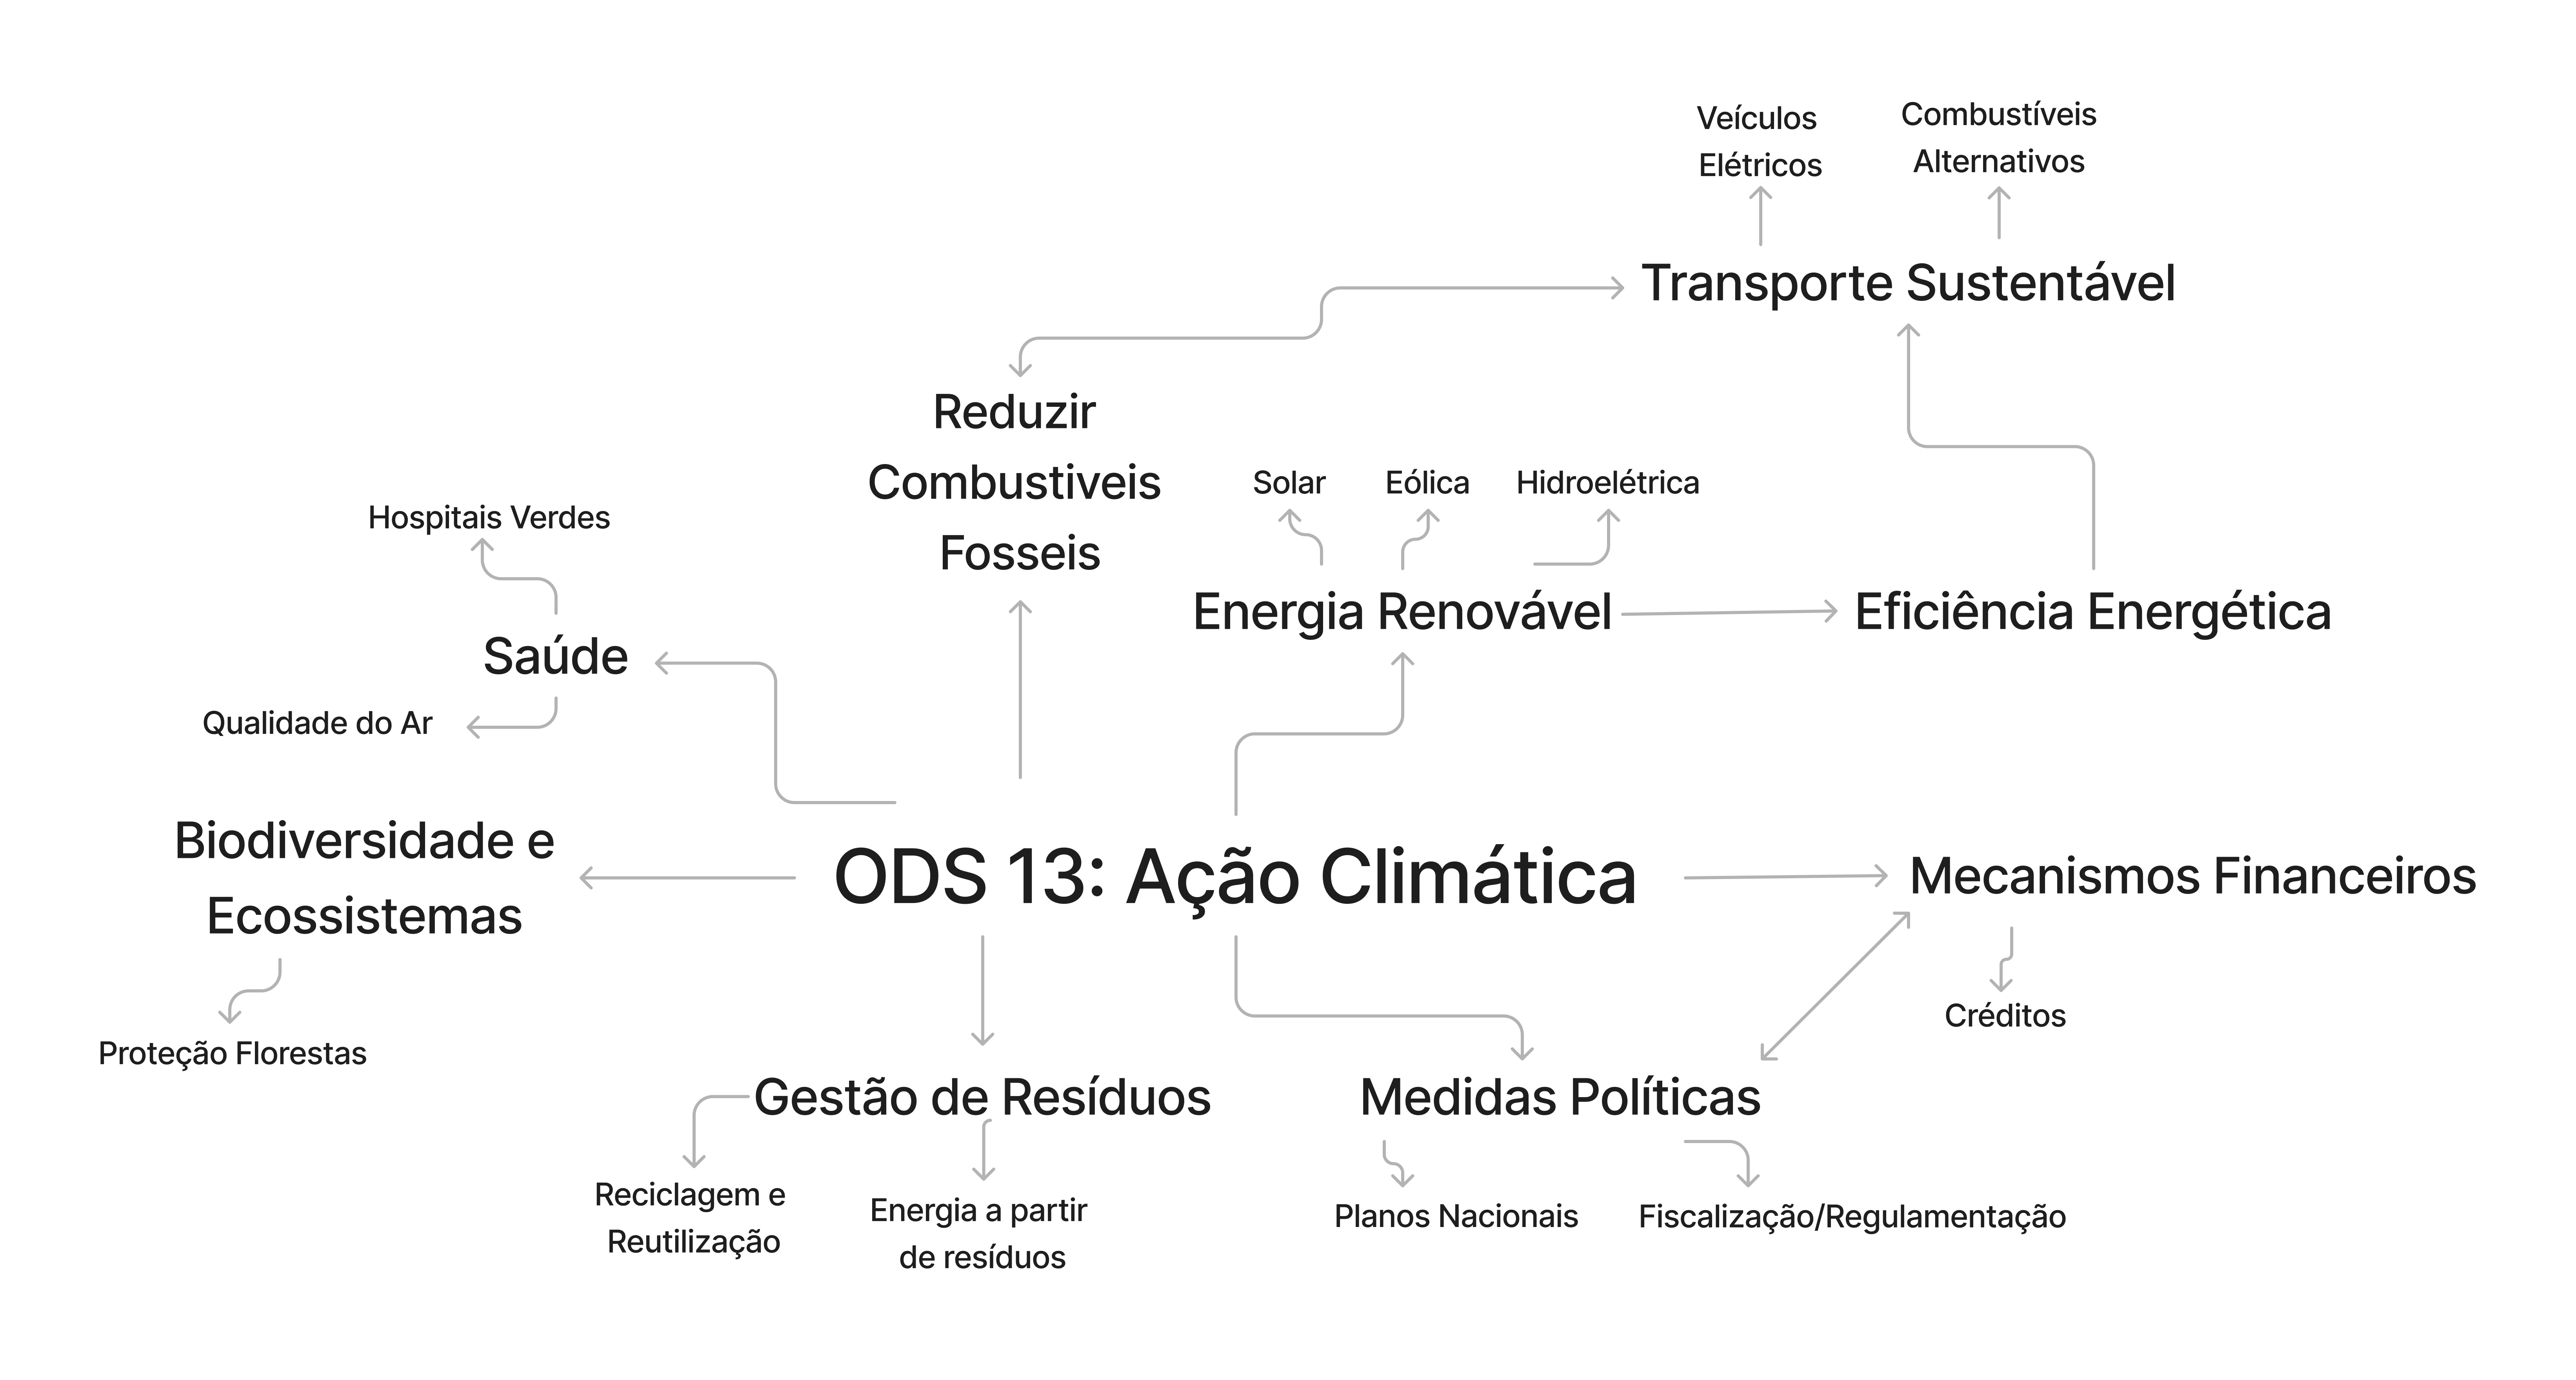
\includegraphics[scale=0.15]{images/opportunity_map.jpg}
    \caption{Mapa de Oportunidade}
    \label{opportunity_map}
\end{figure}

\newpage

Depois do mapa de oportunidade, realizamos um \textit{Intent Statement}\\ Nesta fase foi possível responder aos seguintes tópicos:

\begin{itemize}
    \item \textbf{Problema:} As alterações climáticas, agravadas por eventos extremos, poluição atmosférica (como \ac{gee}) e condições adversas como ondas de calor, tempestades de areia e níveis elevados de poluentes, continuam a impactar negativamente a saúde pública e as infraestruturas urbanas e industriais. As soluções atuais não têm sido eficazes na resposta rápida e adaptável a essas condições.
    %
    \item \textbf{Audiência:} Comunidades urbanas e industriais, principalmente em áreas com condições climáticas extremas ou altos níveis de poluição. Indústrias, autoridades governamentais e gestores de infraestruturas em zonas vulneráveis.
    %
    \item \textbf{Falhanços:} As abordagens anteriores focaram-se na monitorização passiva e em tecnologias caras e complexas de implementação, muitas vezes inadequadas para adaptações rápidas. Além disso, essas soluções falham em responder a múltiplas ameaças climáticas de forma rápida e eficaz.
    %
    \item \textbf{Novo Valor:}  Propomos uma solução modular inovadora com dispositivos que emitem nano partículas para intervir diretamente no clima e na qualidade do ar. Estas partículas realizam ações como a dispersão de partículas anti-alérgicas, neutralização de ácidos na chuva ácida e mitigação de radiação solar em áreas desérticas/de alta temperatura, etc.
    %
    \item \textbf{Oportunidade:} Implementar um sistema sustentável, flexível e de fácil adaptação, capaz de responder a diferentes condições climáticas adversas em tempo real, contribuindo diretamente para a mitigação das mudanças climáticas.
    %
    \item \textbf{Risco:} Desafios relacionados com a escalabilidade do sistema, o custo da implementação a longo prazo, possíveis impactos ecológicos das nano partículas e a dependência da manutenção regular dos dispositivos.
\end{itemize}
%%%%%%
%%%%%%%%%%%
%%%%%%
%%%%%%%%% Empatia %%%%%%%%%
\newpage
\section{Empatia}
Na fase de empatia, apresentamos um mapa de \textit{personas}, no qual são descritos os aspetos comportamentais ao longo do ciclo de vida fictício de um determinado grupo de pessoas:
\begin{figure}[ht]
    \centering
    \begin{minipage}{0.45\textwidth}
        \centering
        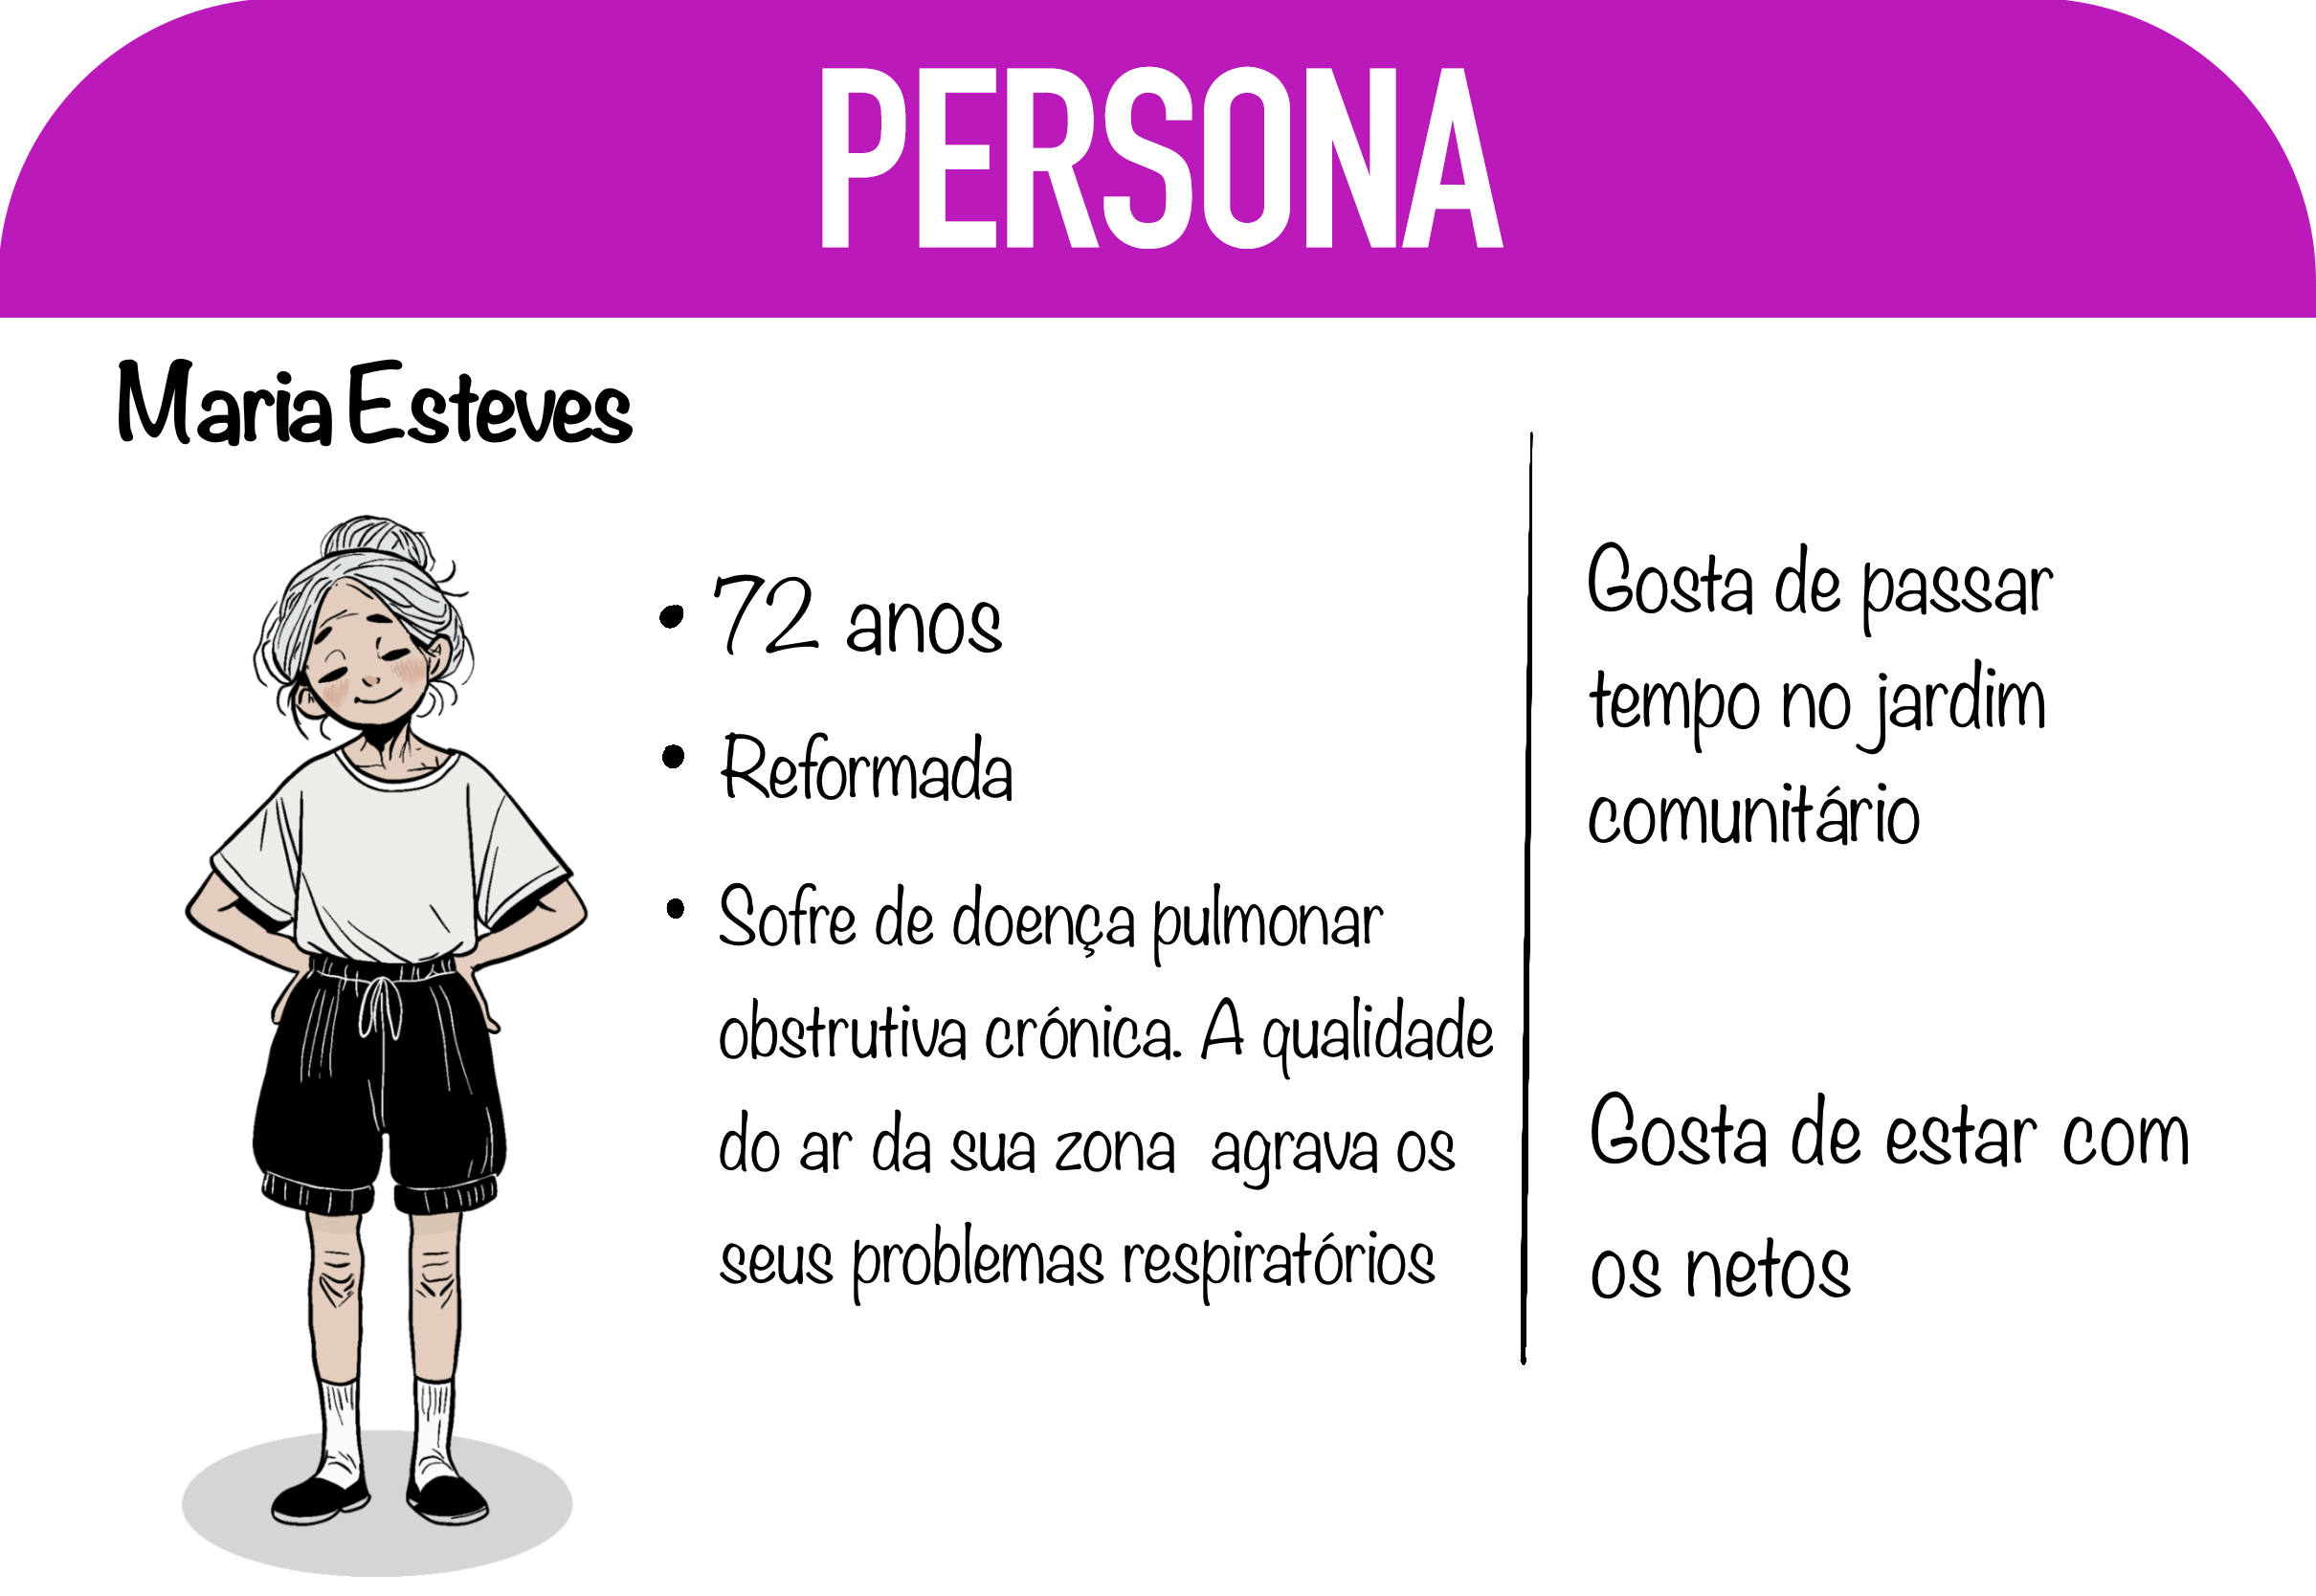
\includegraphics[height=5cm]{images/dona_maria_esteves.png}
        \caption{Persona 1}
        \label{fig:dona_maria_esteves}
    \end{minipage}
    \hfill
    \begin{minipage}{0.45\textwidth}
        \centering
        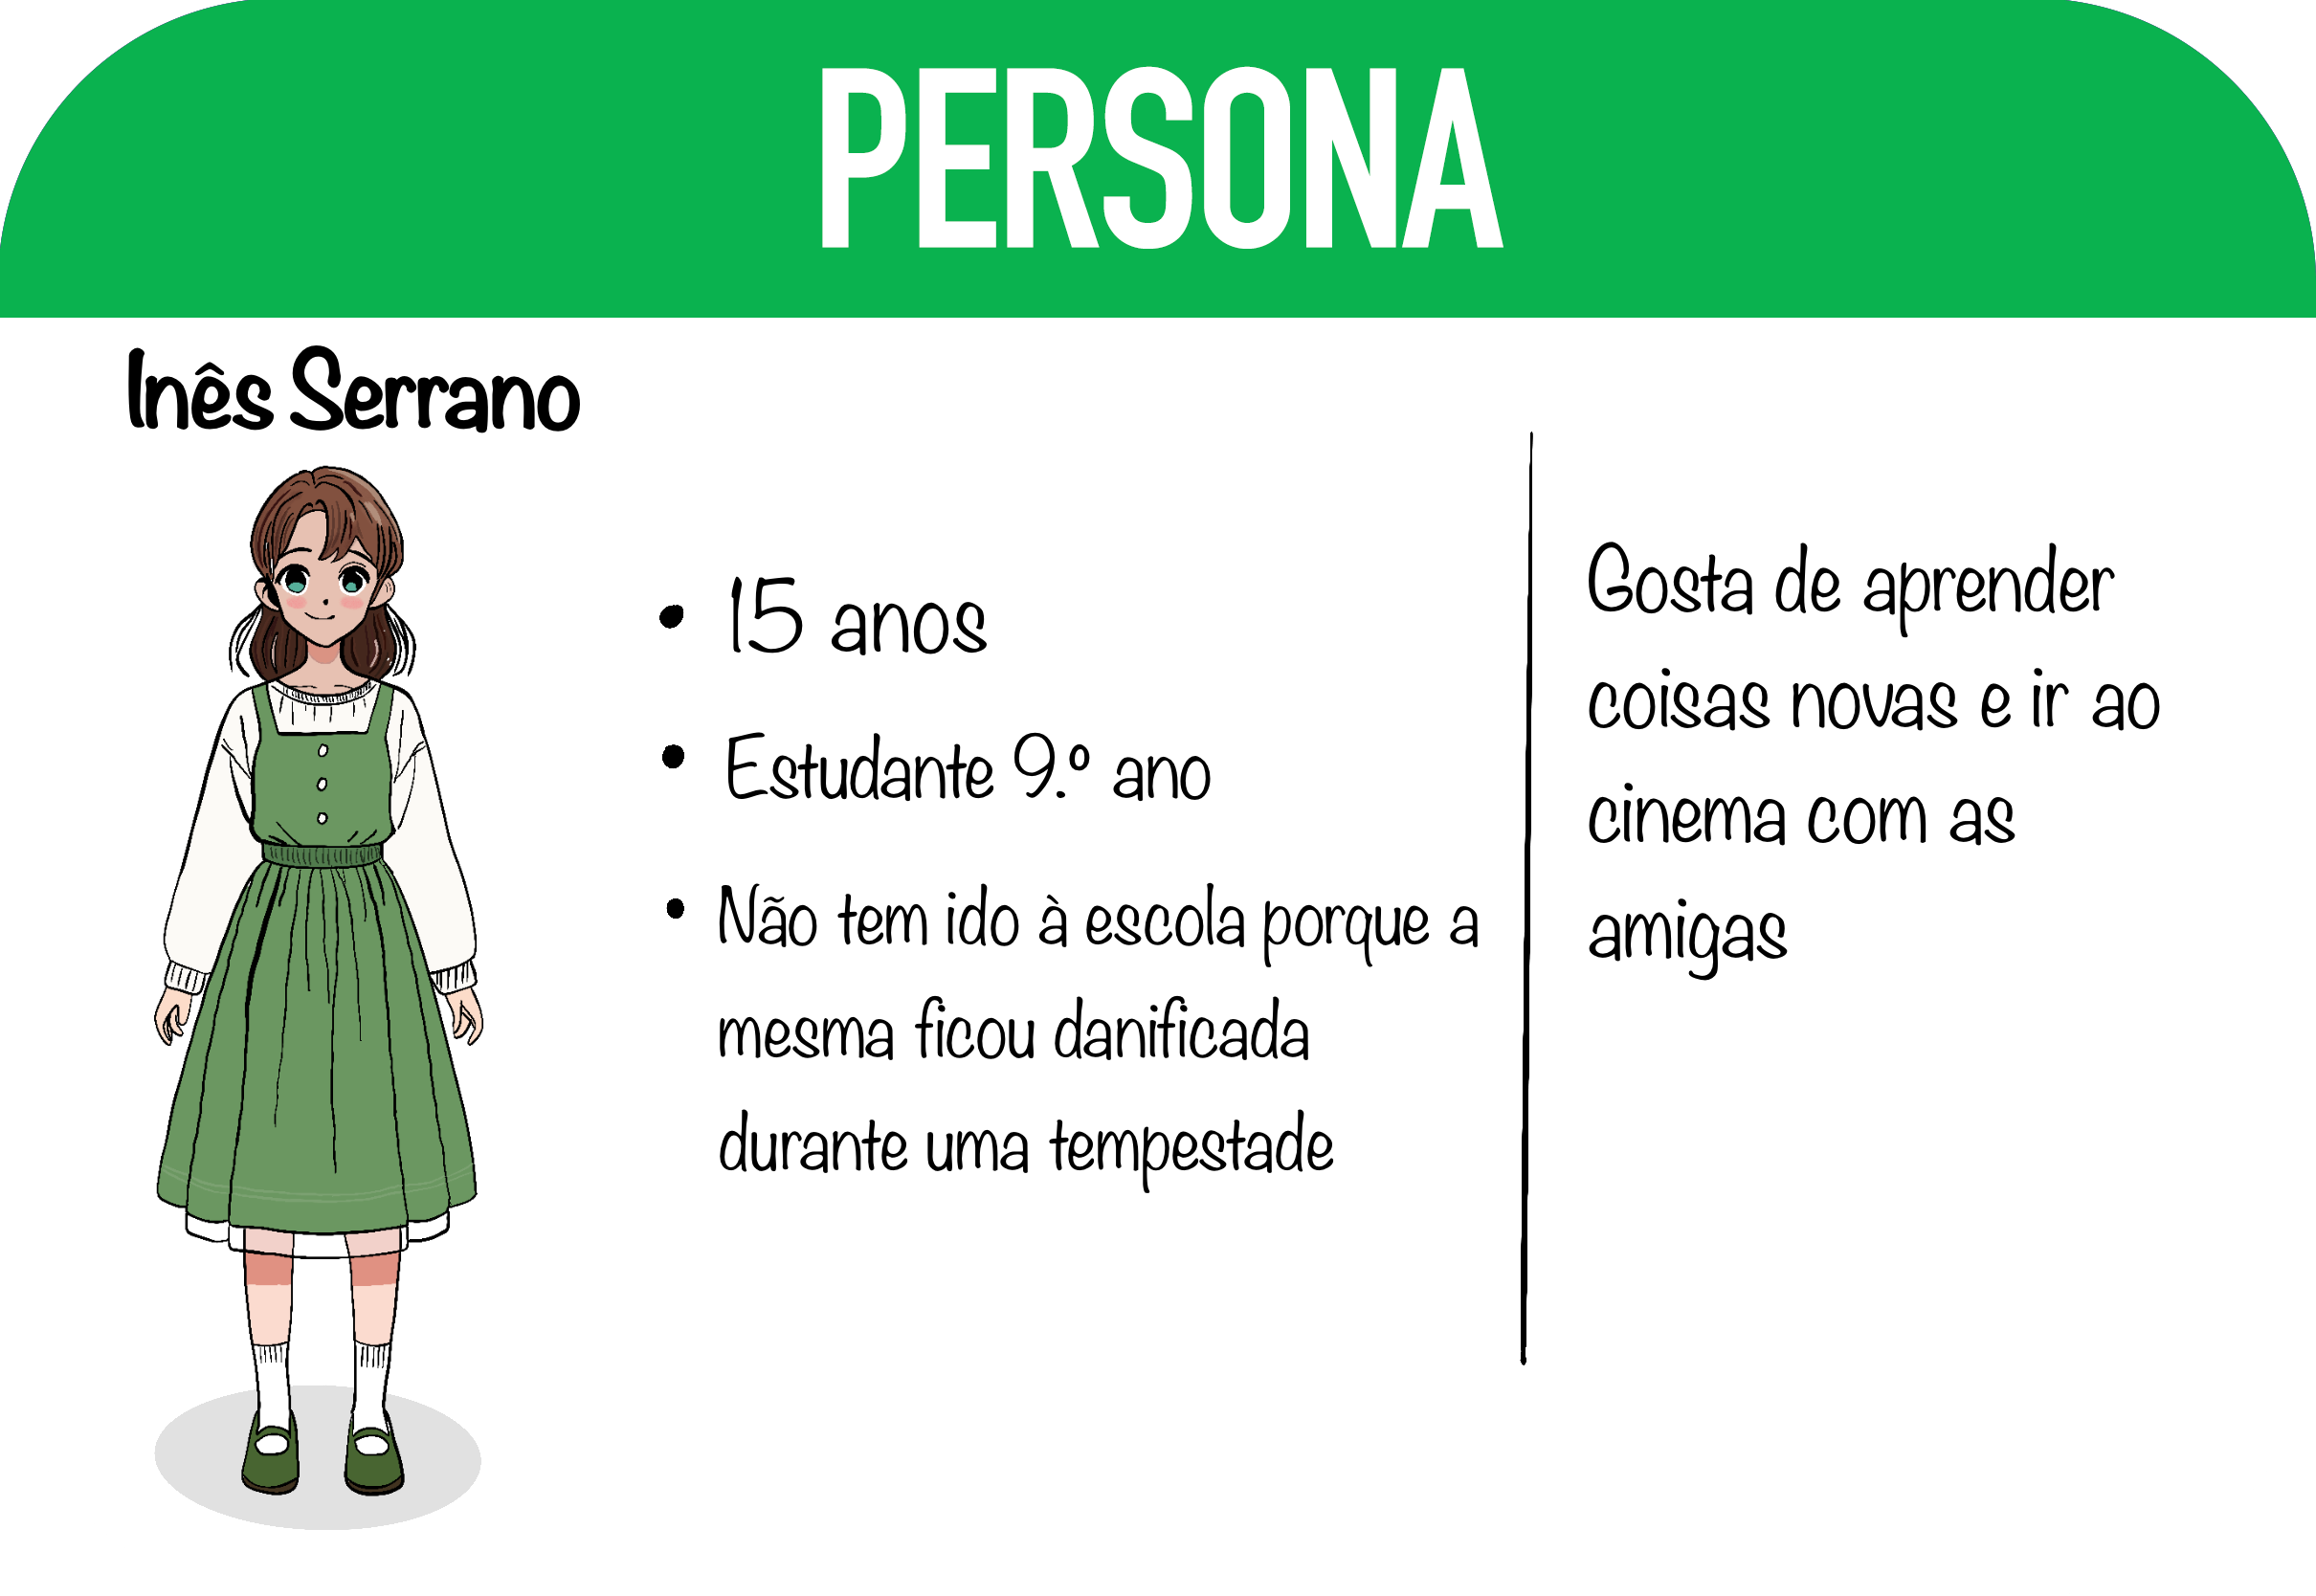
\includegraphics[height=5cm]{images/ines_serrano.png}
        \caption{Persona 2}
        \label{fig:ines_serrano}
    \end{minipage}
\end{figure}

\begin{figure}[ht]
    \centering
    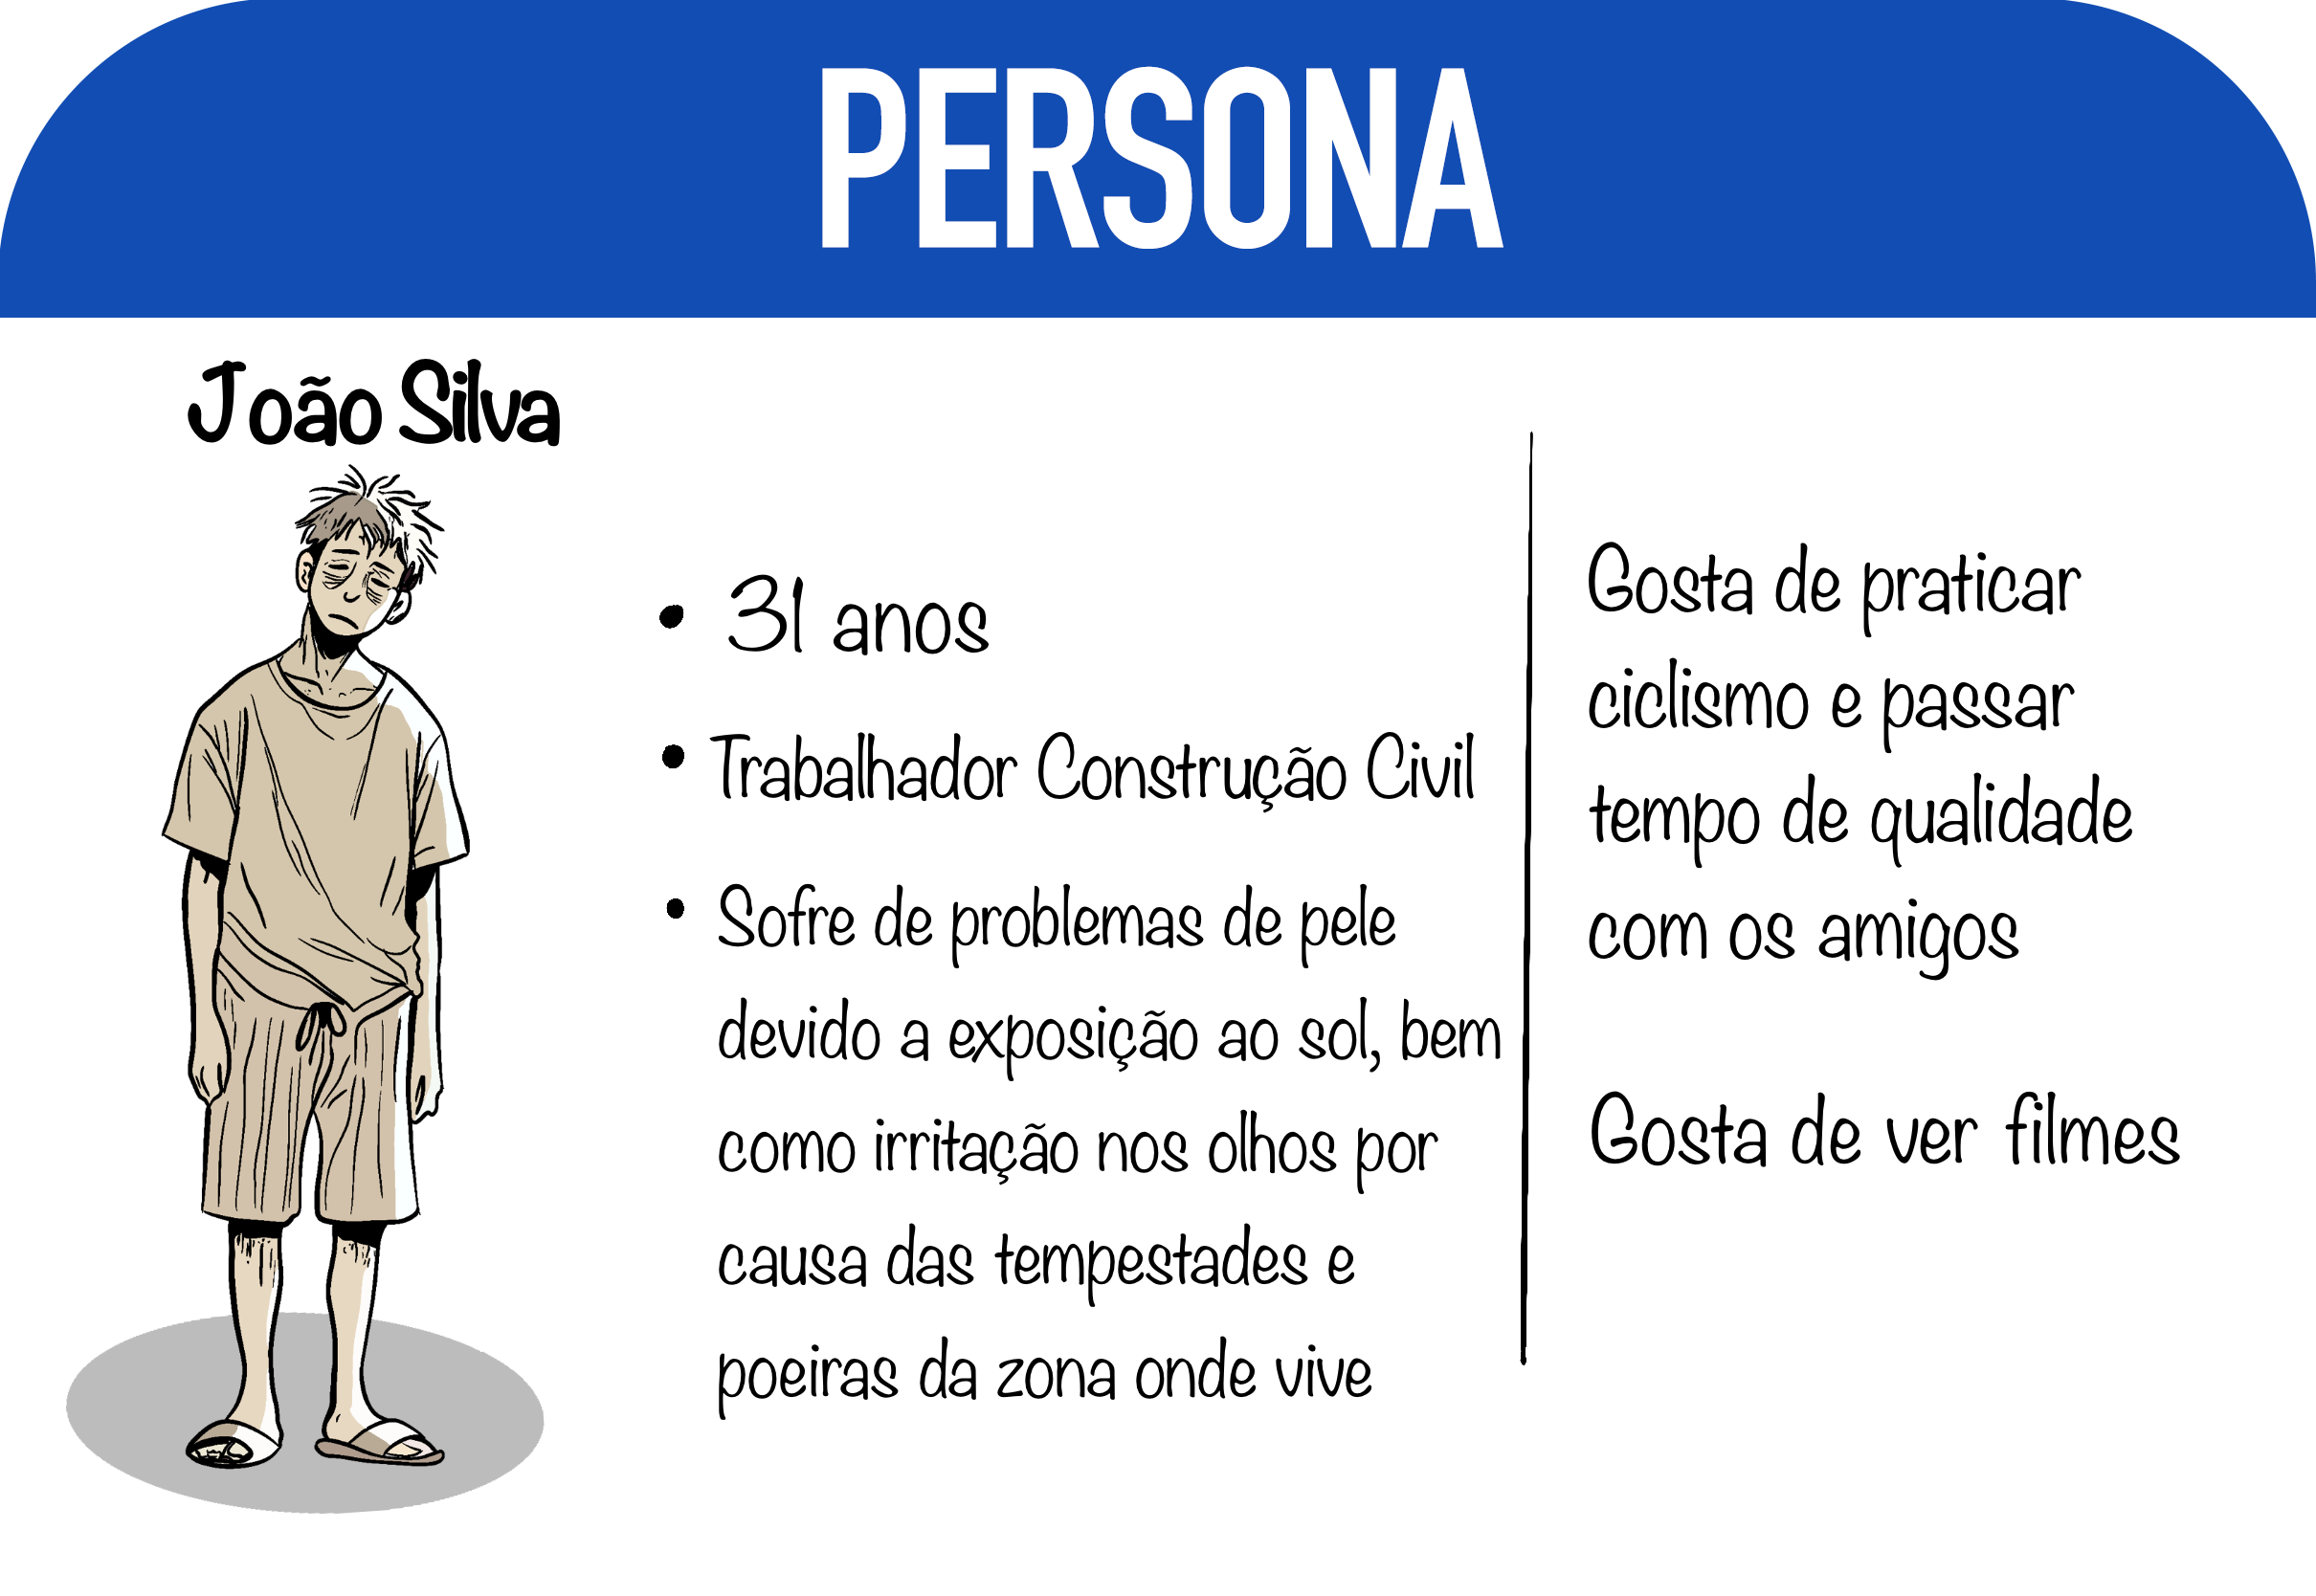
\includegraphics[scale=0.17]{images/joao_silva_png.png}
    \caption{Persona 3}
    \label{fig:joao_silva}
\end{figure}

Na cidade de Vento Leste, as alterações climáticas têm tido um efeito devastador nos últimos anos. As temperaturas médias subiram drasticamente e as tempestades são mais frequentes e intensas. A qualidade do ar piorou, as infraestruturas estão a ceder, e a saúde da população está em risco.
\par
Maria, com 72 anos e reformada, passa os dias a lutar contra os seus problemas respiratórios. O jardim comunitário, que antes era o seu refúgio de paz, agora está coberto de poeira e resíduos deixados pelas tempestades de areia. Maria sente-se isolada, pois já não consegue passar tanto tempo ao ar livre ou a brincar com os seus netos como antes.
\par
Inês, uma estudante de 15 anos, deixou de ir à escola depois que o edifício escolar foi gravemente danificado por uma tempestade. Com a interrupção das aulas presenciais, Inês teve que adaptar-se às aulas online, mas o acesso à internet é inconsistente. Ela sente-se desmotivada, pois já não tem o contacto diário com as suas amigas.
\par
João, um trabalhador da construção civil de 31 anos, está a enfrentar uma nova realidade difícil. As temperaturas elevadas e a exposição prolongada ao sol estão a piorar as suas condições de trabalho, e ele tem sofrido com irritações graves na pele. Sente-se cada vez mais exausto física e mentalmente, pois vê a sua qualidade de vida degradar-se em ritmo acelerado.

%%%%%%
%%%%%%%%%%%
%%%%%%
%%%%%%%%% Experimentação %%%%%%%%%
\section{Experimentação}
Durante a fase de experimentação, explorámos uma ampla variedade de ideias utilizando técnicas como \textit{brainstorming\footnote{Técnica que visa propor soluções criativas para problemas específicos}}. O principal recurso criativo foi o desenvolvimento de um mapa de ideias (Figura \ref{fig:mapa_ideias}).

\begin{figure}[ht]
    \centering
    \includegraphics[scale=0.10]{images/mapa_ideias.jpg}
    \caption{Mapa de ideias - \href{https://imgur.com/a/ULVbBdO}{\underline{link para imagem com maior resolução}}}
    \label{fig:mapa_ideias}
\end{figure}

Tendo em conta que o principal tema eram alterações climáticas pensamos nas analogias seguintes:

\begin{itemize}
    \item \textbf{\textit{Reverse Analogy: }} Sendo o tema Ações/Alterações Climáticas, uma analogia reversa seria não existirem mudanças climáticas. Um caso, onde não haveriam quaisquer problemas climáticos, ou consequências dos mesmos.

    \item \textbf{\textit{Direct Analogy: }}Assim como um sistema de filtragem de água remove impurezas e toxinas da água, poderiam existir dispositivos que atuassem da mesma forma regulando condições climáticas.
    
\end{itemize}

Ao longo do processo criativo, explorámos várias ideias que nos ajudaram a chegar ao conceito atual. Inicialmente, considerámos \textbf{edifícios que captariam e utilizariam o \coo}, mas rapidamente percebemos que essa solução era inviável. Depois, pensámos em \textbf{Tintas Biológicas} com microrganismos, uma alternativa barata e eficiente às tintas comuns, mas durante a pesquisa descobrimos que a ideia já existia.
\par
Também cogitámos um sistema de distorção temporal para \textbf{retardar os efeitos das alterações climáticas} usando torres interligadas, mas a complexidade científica fez-nos repensar. Estas experiências culminaram no nosso conceito atual das nano partículas, que reúne os aspetos mais promissores das ideias anteriores numa solução prática e eficiente.

\newpage
%%%%%%
%%%%%%%%%%%
%%%%%%
%%%%%%%%% Elaboração %%%%%%%%%
\section{Elaboração}
Após diversas sessões de brainstorming e análises, concluímos que a melhor solução para enfrentar os desafios climáticos seria uma abordagem tecnológica, flexível e adaptável. Surgiu, assim, a ideia de desenvolver dispositivos modulares que, instalados em infraestruturas urbanas ou industriais, emitiriam partículas nanoestruturadas capazes de interagir com o ambiente, neutralizar poluentes e mitigar eventos climáticos severos, contribuindo para a saúde pública e para a adaptação às mudanças climáticas.

\begin{figure}[ht]
    \centering
    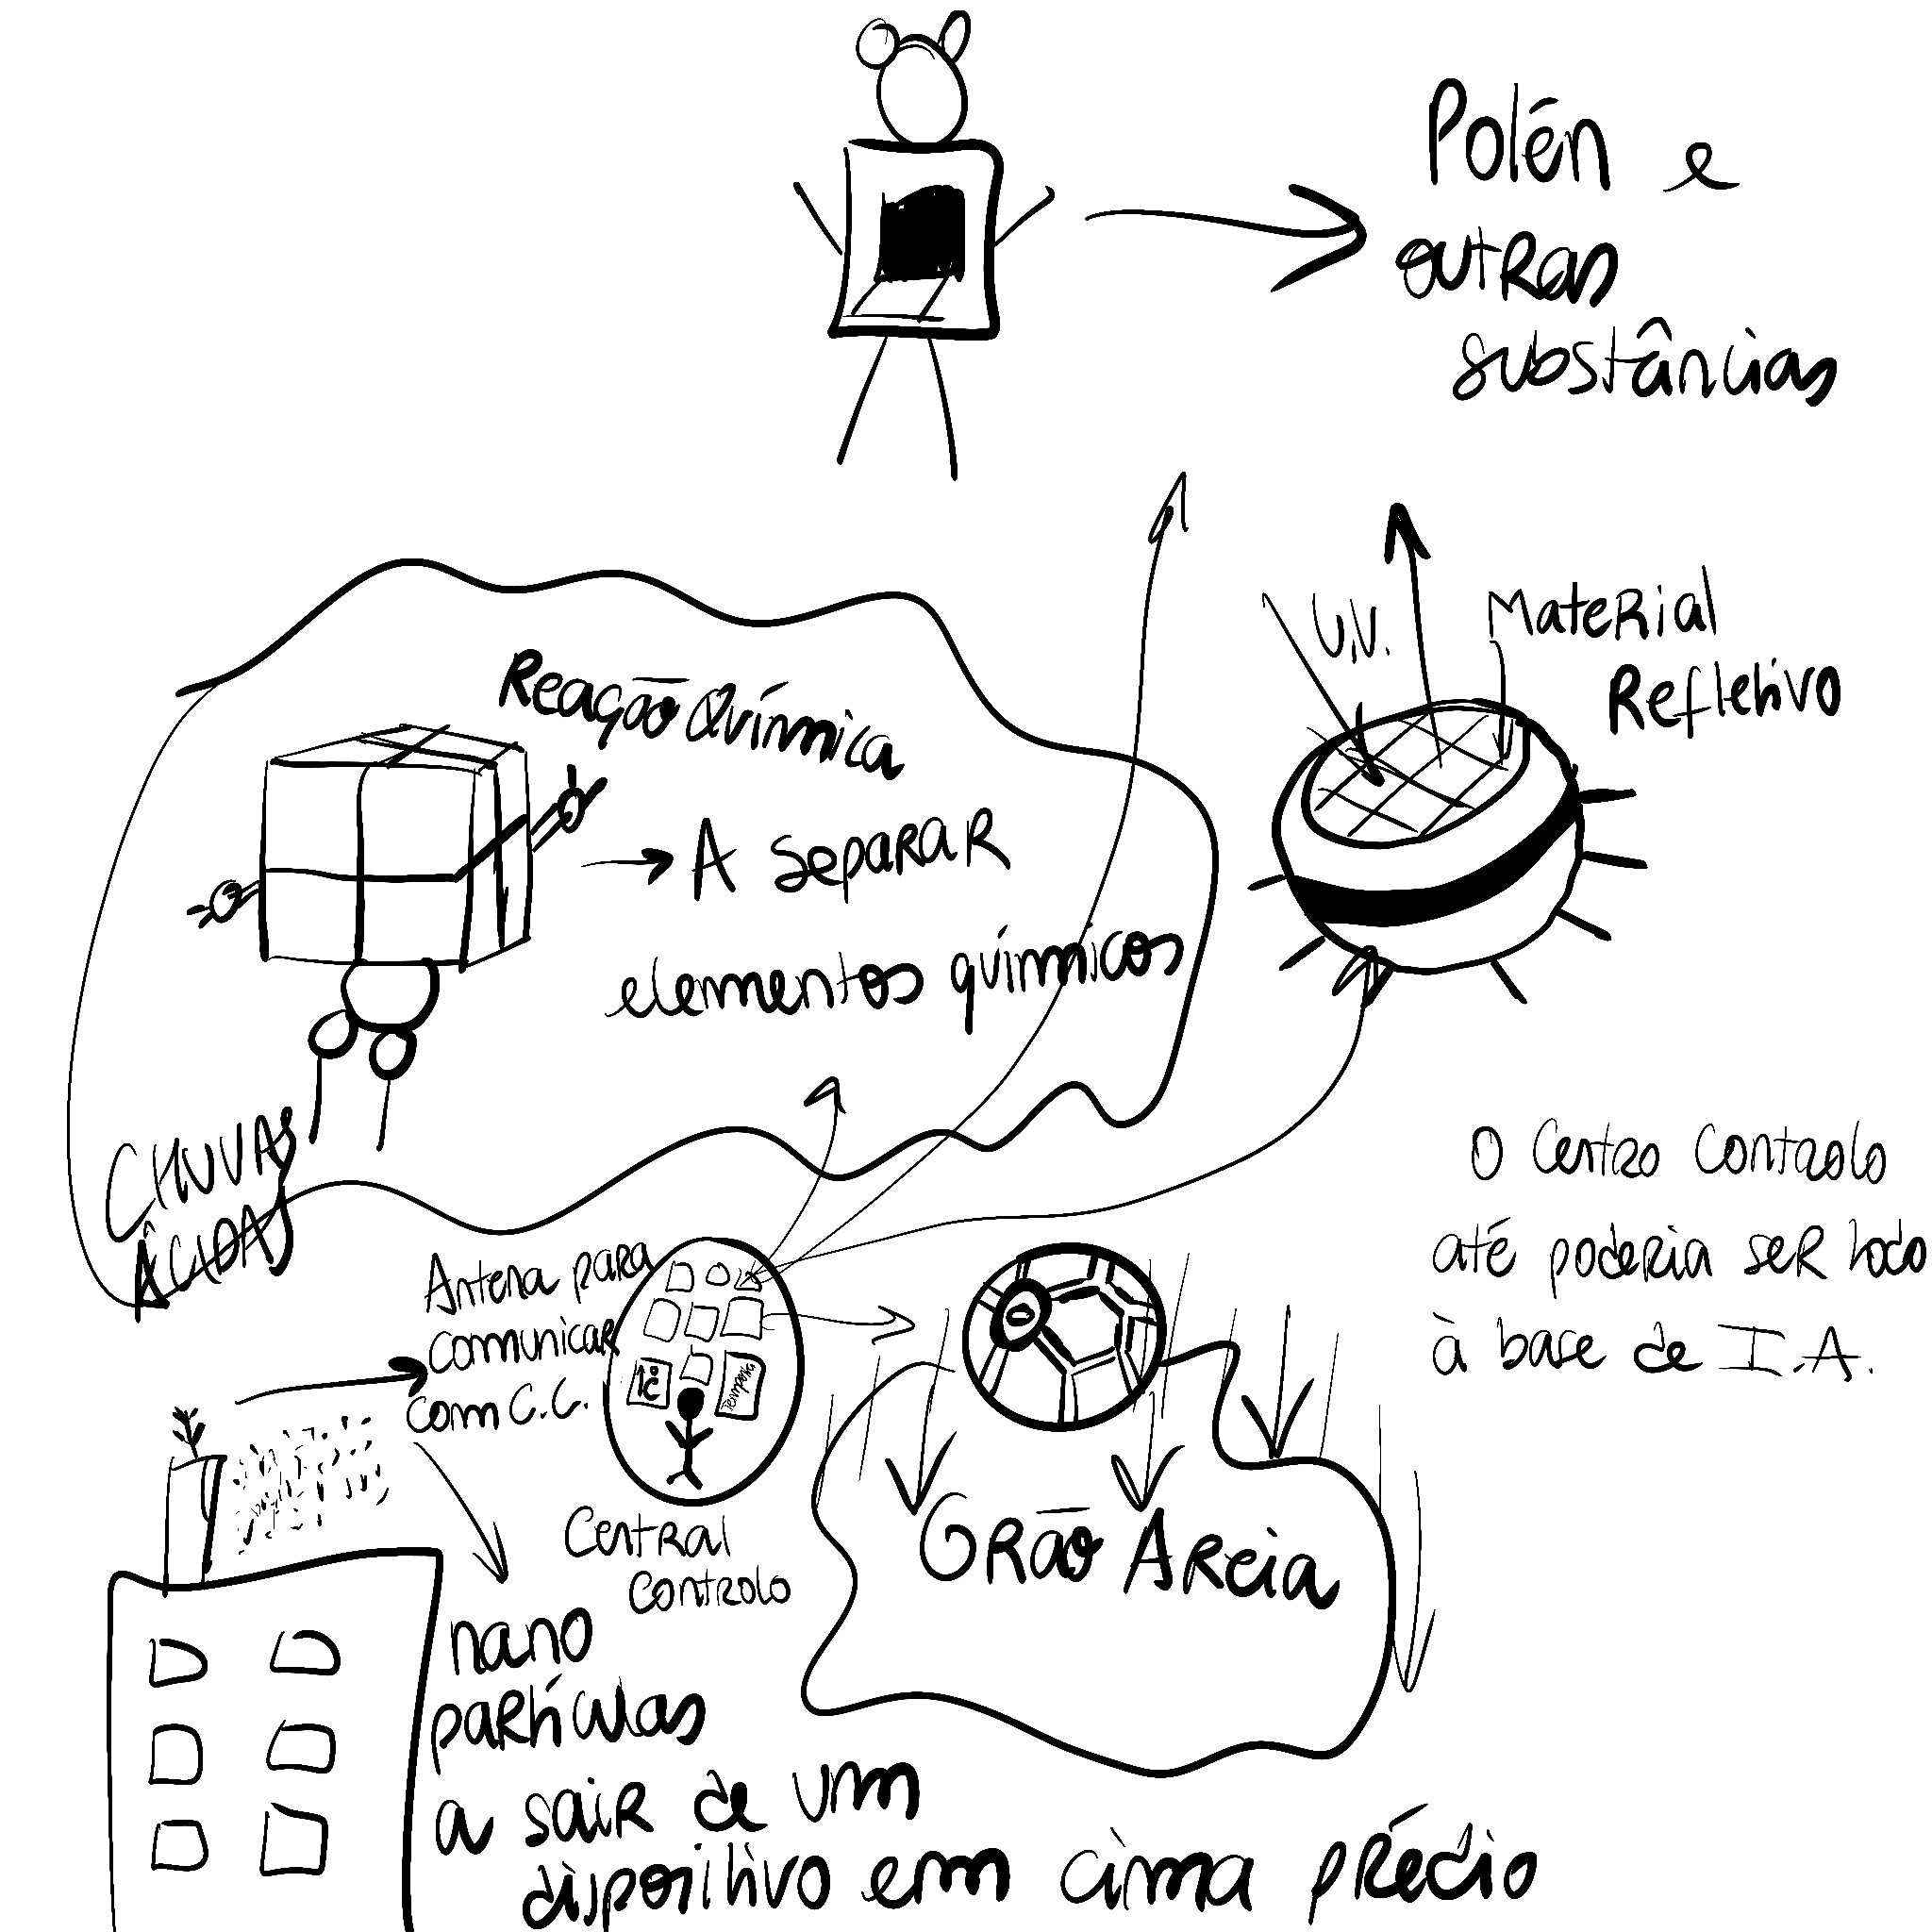
\includegraphics[scale=0.13]{images/esboco_inicial.jpg}
    \caption{Esboço Inicial}
    \label{fig:esboco_inicial}
\end{figure}

%%%%%%
%%%%%%%%%%%
%%%%%%
%%%%%%%%% Exposição %%%%%%%%%
\section{Exposição}
O projeto de dispositivos modulares com \textbf{nano-partículas} oferece uma solução inovadora para os desafios das alterações climáticas. Instalados em infraestruturas altas, como torres ou edifícios, estes dispositivos monitorizam e intervêm no ambiente, utilizando tecnologias avançadas. Controlados por um sistema de Inteligência Artificial (IA), analisam em tempo real a qualidade do ar e condições atmosféricas, ajustando automaticamente a resposta às necessidades ambientais.
%%%%%%%%%%% Monitorização e Emissão de Nano-partículas %%%%%%%%%%
   
\subsection{Monitorização e Emissão de Nano-partículas}
Estas nano-partículas desempenham um papel crítico na captura de poluentes atmosféricos e na mitigação de condições adversas. Funções como a neutralização de ácidos na chuva (Figura \ref{fig:chuvas_acidas}), o controlo de partículas alergénicas e a redução de radiação solar em zonas desérticas ou com temperaturas extremas (Figura \ref{fig:high_temperatures}) são algumas das intervenções possíveis.
\begin{figure}[ht]
    \centering
    \begin{minipage}{0.45\textwidth}
        \centering
        \fbox{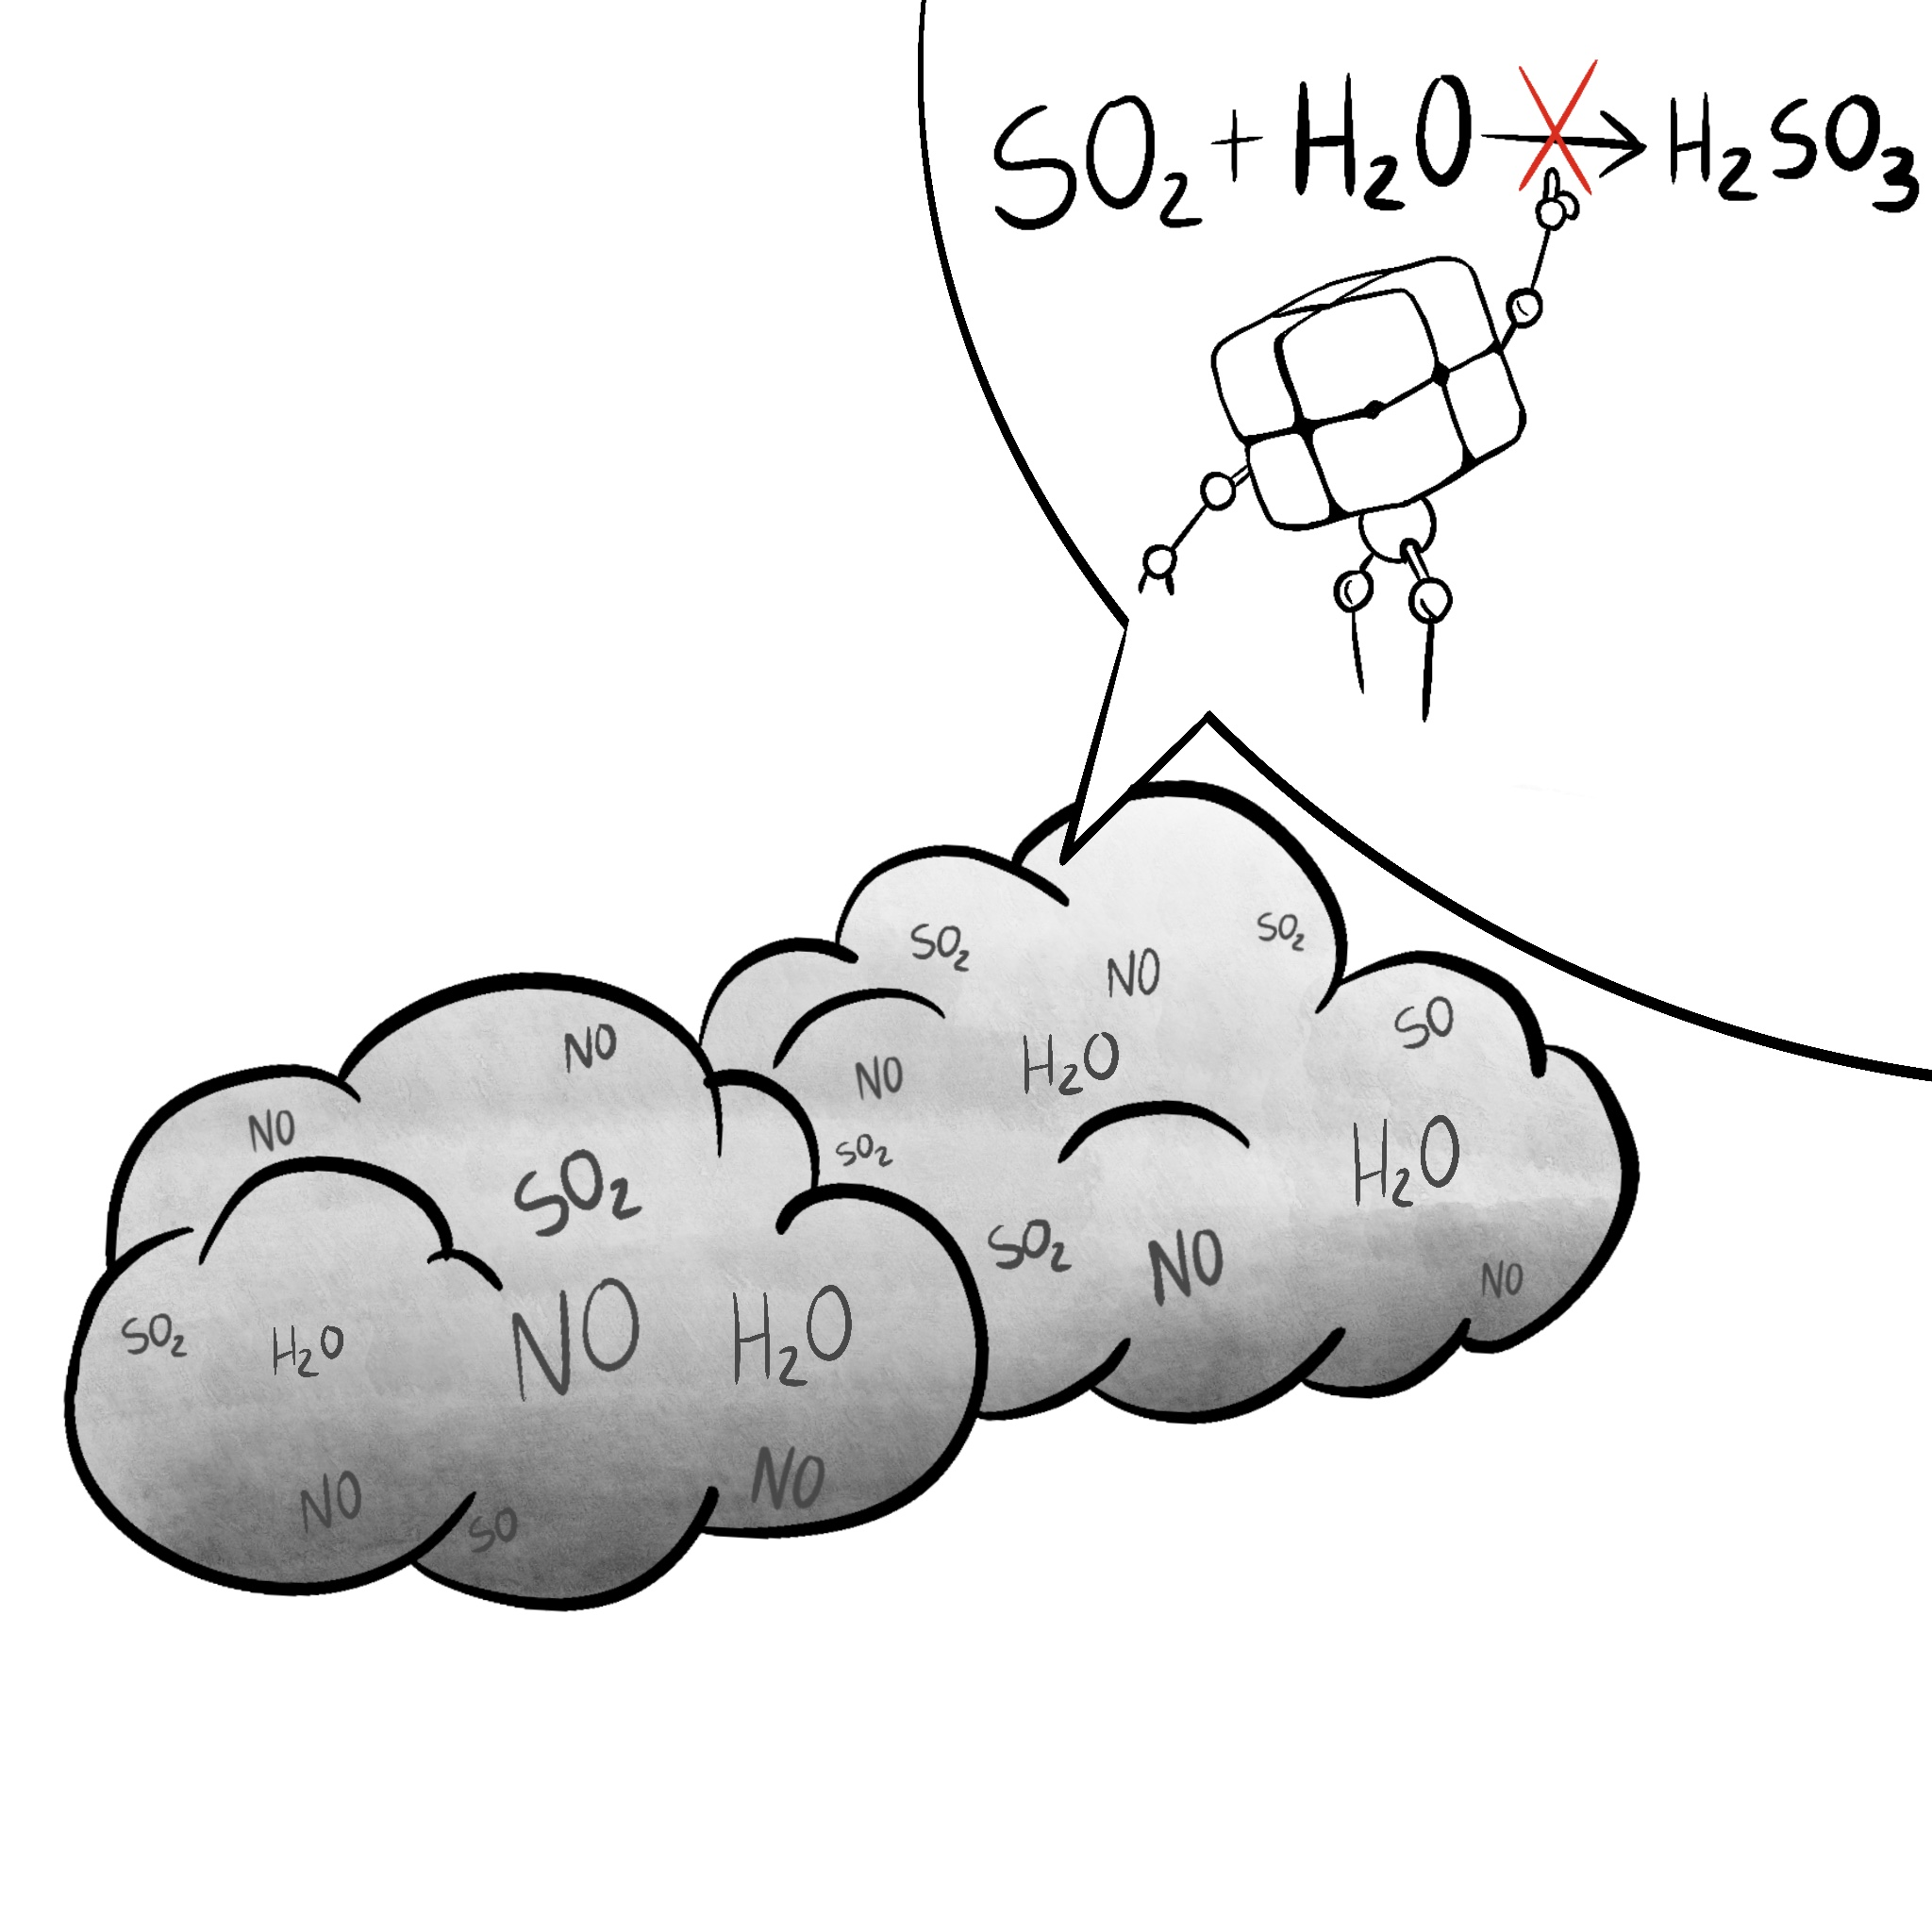
\includegraphics[height=6cm]{images/chuvas_acidas.jpg}}
        \caption{Nano partícula a quebrar a reação química}
        \label{fig:chuvas_acidas}
    \end{minipage}
    \hfill
    \begin{minipage}{0.45\textwidth}
        \centering
        \fbox{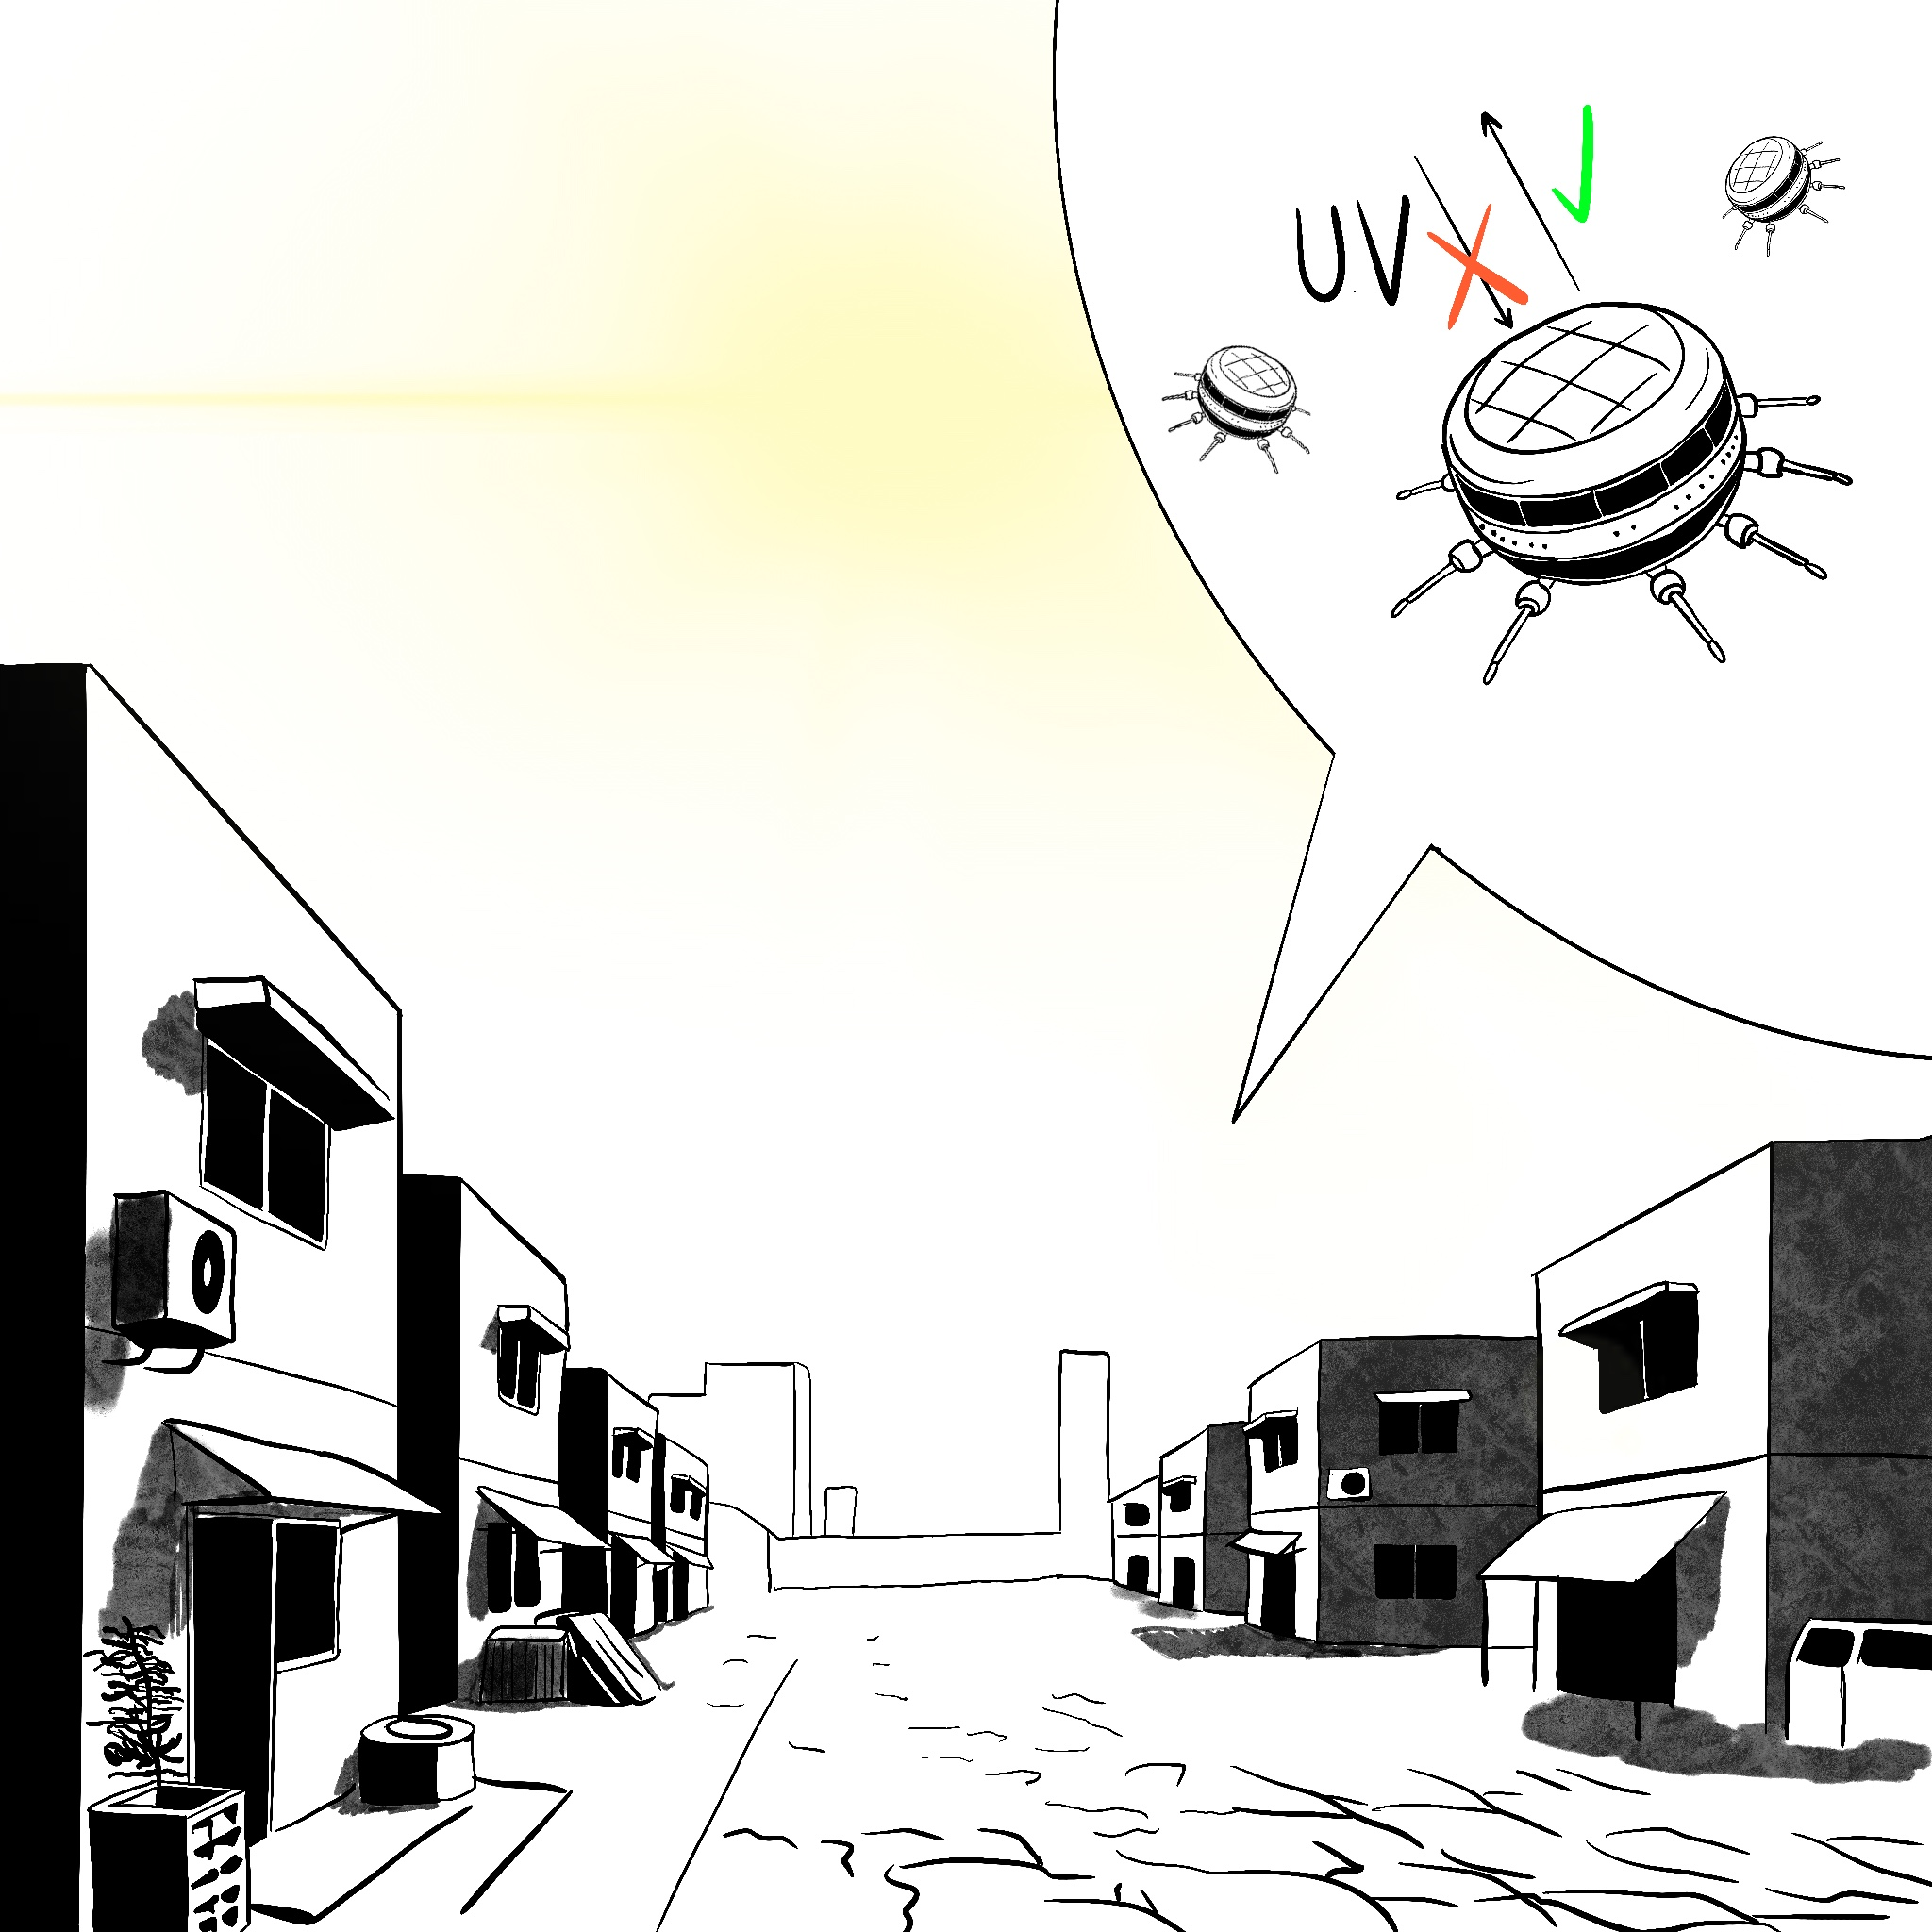
\includegraphics[height=6cm]{images/high_temperatures.jpg}}
        \caption{Nano partícula a refletir raios \ac{uv}}
        \label{fig:high_temperatures}
    \end{minipage}
\end{figure}

%vspace

%%%%%%%%%%% Mitigação de Eventos Climáticos %%%%%%%%%%
\subsection{Mitigação de Eventos Climáticos Severos}

\begin{figure}[h!]
    \centering
    \begin{minipage}{0.45\textwidth}
        \fbox{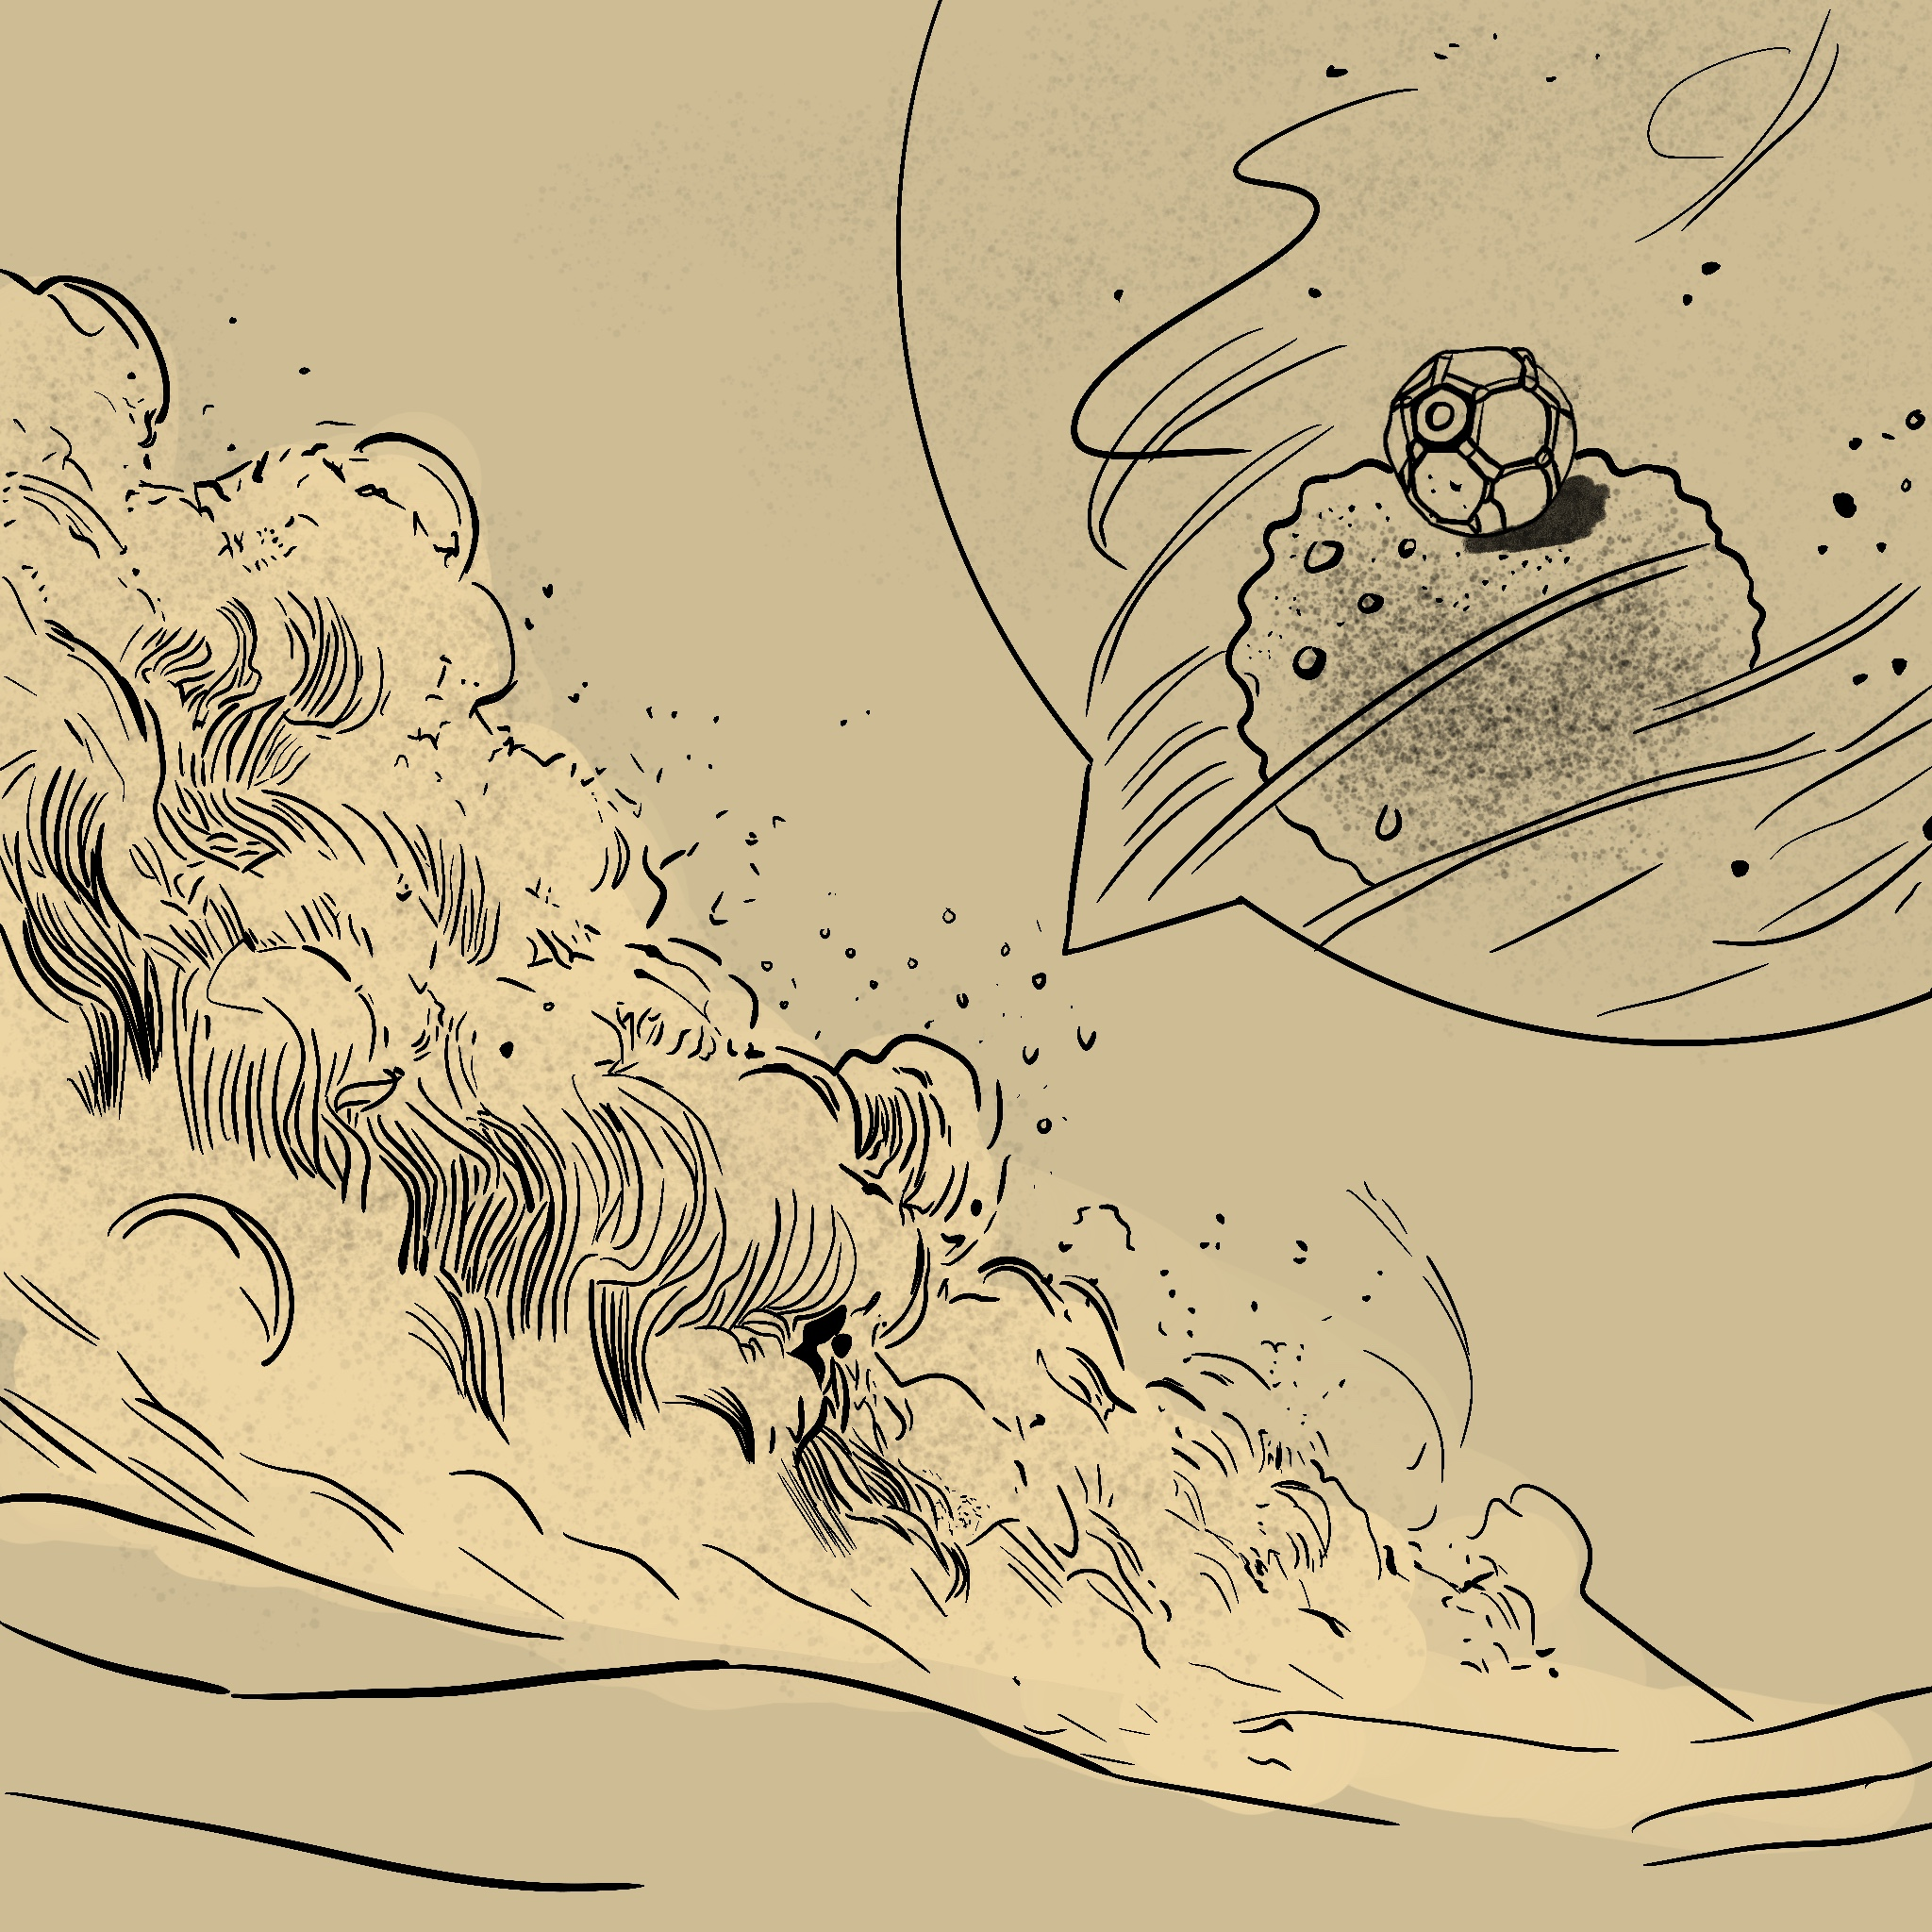
\includegraphics[height=6cm]{images/sandstorm.jpg}}
        \caption{Nano partícula em cima de um grão de areia, numa tempestade.}
        \label{fig:sandstorm}
    \end{minipage}
    \hfill
    \begin{minipage}{0.5\textwidth}
    \vspace{-1cm}
        Um papel importante das nano partículas é também a \textbf{mitigação de tempestades de areia}. Em regiões propensas a este tipo de fenómenos, as nano partículas são capazes de se afixar às partículas de poeira, tornando-as mais pesadas e acelerando o seu assentamento no solo. Isso reduz o impacto na visibilidade e melhora a qualidade do ar (Figura \ref{fig:sandstorm}).
    \end{minipage}
\end{figure}

%%%%%%%%%%%%%%%%%%%%%%%%%%%%%%%% Resultado %%%%%%%%%%%%%%%%%%%%%%%%%%%%%%%%
\chapter{Resultado}
\label{chap.resultado}
Os dispositivos modulares que hospedam as nano-partículas quando estão inativas, encontram-se em lugares altos, como torres de alta tensão, edifícios ou infraestruturas urbanas. Os dispositivos, em comunicação com uma central capaz de analisar situações como a qualidade do ar ou identificar situações críticas, são capazes de identificar a necessidade de intervenção.
\par
Quando identificam a necessidade de intervenção, os dispositivos emitem as \textbf{nano partículas} específicas para a resolução do problema em causa: 
\begin{itemize}
    \item \textbf{Controlo de ácidos, alergénicos e gases poluentes}.
    \item \textbf{Aderir a partículas de poeira em tempestades de areia, facilitando a sua deposição no solo}.
    \item \textbf{Controlo de radiação solar para reduzir temperaturas}.
\end{itemize}

\begin{figure}[ht]
    \centering
    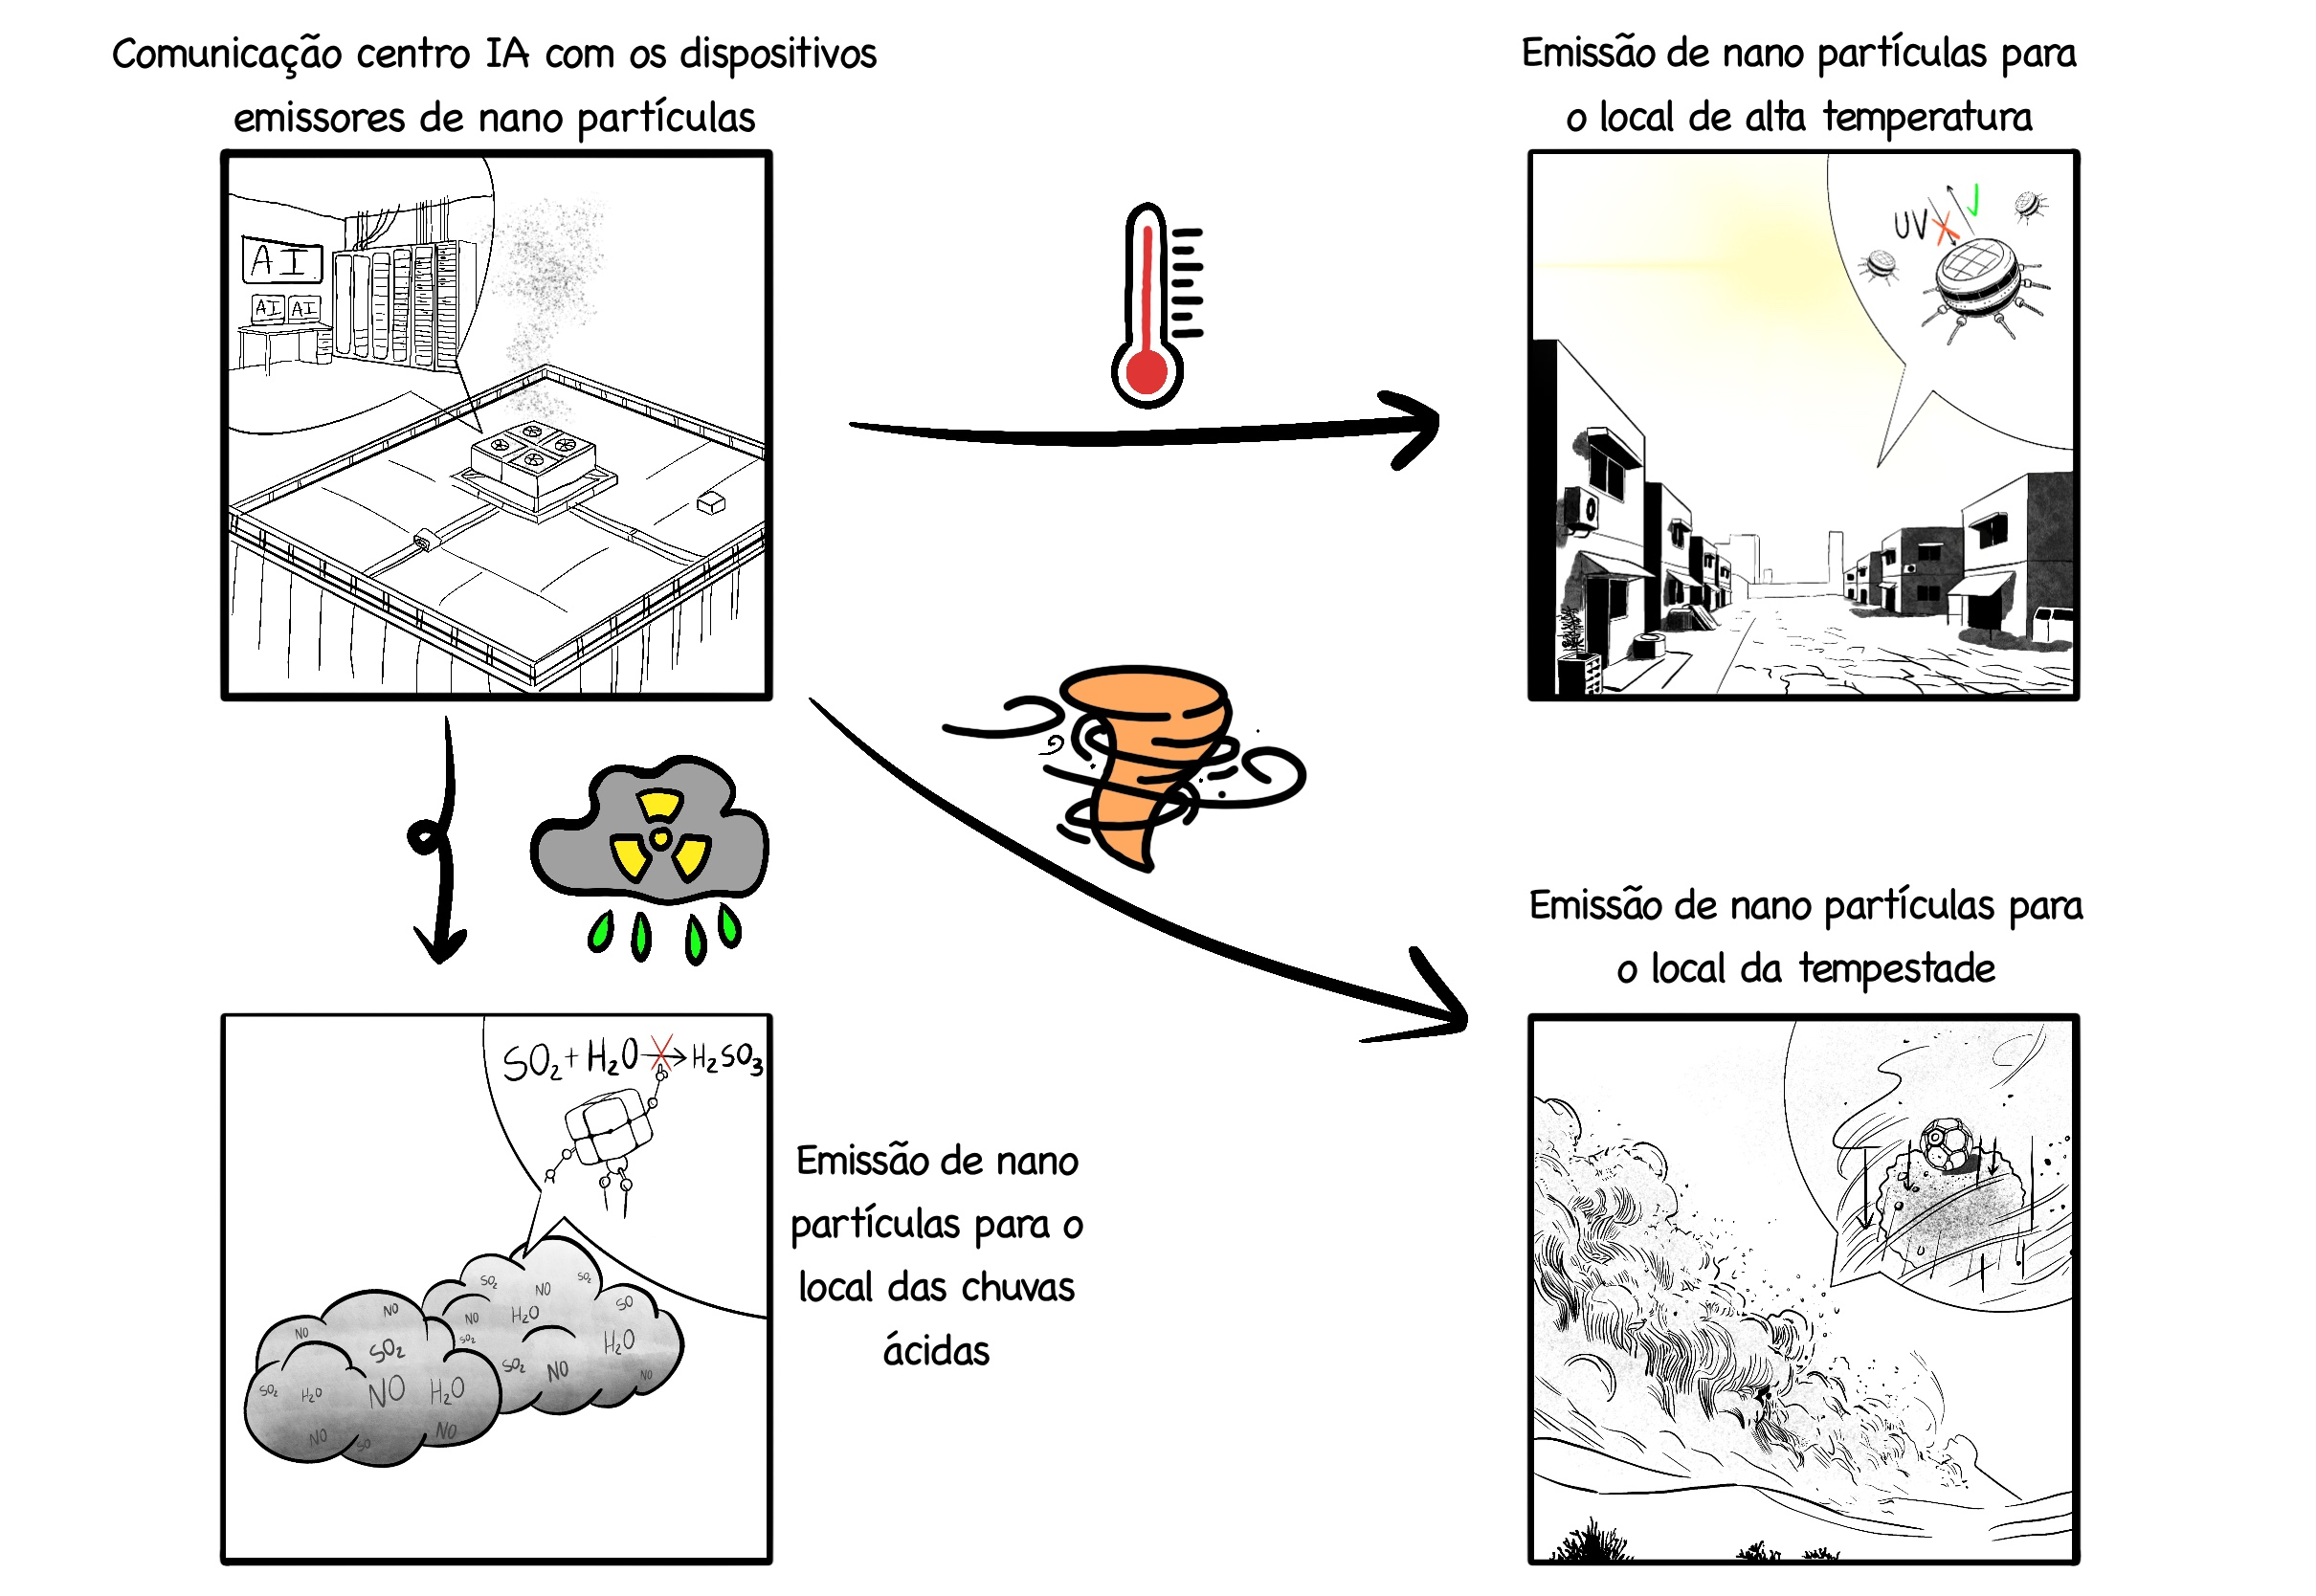
\includegraphics[scale=0.17]{images/result.jpg}
    \caption{Resultado}
    \label{fig:result}
\end{figure}



%%%%%%%%%%%%%%%%%%%%%%%%% Reflexão Final %%%%%%%%%%%%%%%%%%%%%%%%%%%%%%%%%
\chapter{Reflexão Final}
\label{chap.reflexaoFinal}
O processo criativo deste projeto foi uma experiência de grande aprendizagem, onde a exploração de ideias inovadoras e a busca por soluções práticas andaram lado a lado. O uso de técnicas como brainstorming e métodos de divergência e convergência permitiu-nos ampliar a nossa visão inicial, ajudando a identificar possibilidades que inicialmente não considerávamos.
\par
Um dos principais desafios foi arranjar um equilíbrio entre a criatividade e a viabilidade técnica das propostas. Em várias fases, tivemos de abandonar ideias que, embora inovadoras, não poderiam ser sustentadas de forma prática.
\par
Ainda assim, as técnicas de brainstorming e de divergência e convergência ajudaram-nos a explorar um leque amplo de possibilidades antes de nos focarmos numa direção específica. No entanto este processo também exigiu lidar com a incerteza e a ambiguidade, que fazem parte da jornada criativa. Foi preciso "aprender" a conviver com a ausência de respostas concretas e a confiar mais no processo de experimentação, sabendo que algumas ideias apenas mostrariam o seu potencial (ou falta dele) depois de serem testadas.
\par
Para concluir, o trabalho de equipa e a troca de perspetivas foram elementos fulcrais para o sucesso do projeto. Em última análise, a metodologia de \textit{Design Thinking} revelou-se uma oportunidade única para desenvolver novas formas de pensar, superar problemas e incertezas, e de avançar de forma mais confiante.
\par  
Aprendemos que a inovação não é apenas ter boas ideias, mas também saber adaptá-las e trabalhar em conjunto para torná-las realidade


%%%%%%%%%%%%%%%%%%%%%%%%%%%%%%%%%
\chapter*{Acrónimos}
\begin{acronym}
\acro{ua}[UA]{Universidade de Aveiro}
\acro{gee}[GEE]{Gases do Efeito de Estufa}
\acro{ia}[IA]{Inteligência Artificial}
\acro{uv}[U.V]{Ultra Violeta}
\end{acronym}
%%%%%%%%%%%%%%%%%%%%%%%%%%%%%%%%%

\begin{flushright}
    \today
\end{flushright}

\printbibliography
\end{document}